\newcommand{\name}{E207 -- Lab course Accelerator Bonn (LAB) }
\documentclass[11pt,a4paper,notitlepage]{scrartcl}
\usepackage{DasPaket}
\title{ Advanced Laboratory Course}
\subtitle{\name  \\ \hrulefill}
\date{March 31 2021 \\ }
%\date{Date of Experiment \\ \sectionlinetwo{black}{88}}
\author[*]{\textsc{Dominic Schüchter}}
\author[$\dagger$]{\textsc{Jakob Krause}}
\affil[*]{\href{mailto:dschuechter@uni-bonn.de}{\faEnvelope  \hspace*{0.1cm}dschuechter@uni-bonn.de} {\color{black}$|$} \href{https://github.com/dschuechter}{\faGithub  \hspace*{0.1cm}dschuechter}}
\affil[$\dagger$]{\href{mailto:krause.jakob@uni-bonn.de}{\faEnvelope  \hspace*{0.1cm}krause.jakob@uni-bonn.de} {\color{black}$|$} \href{https://github.com/krausejm}{\faGithub  \hspace*{0.1cm}krausejm}}
\usepackage{blindtext}
\usepackage{booktabs}

\graphicspath{{figs/}}
\addbibresource{Literatur.bib}


\begin{document}

\maketitle
\vspace{-.8cm}
\thispagestyle{empty}
\begin{center}
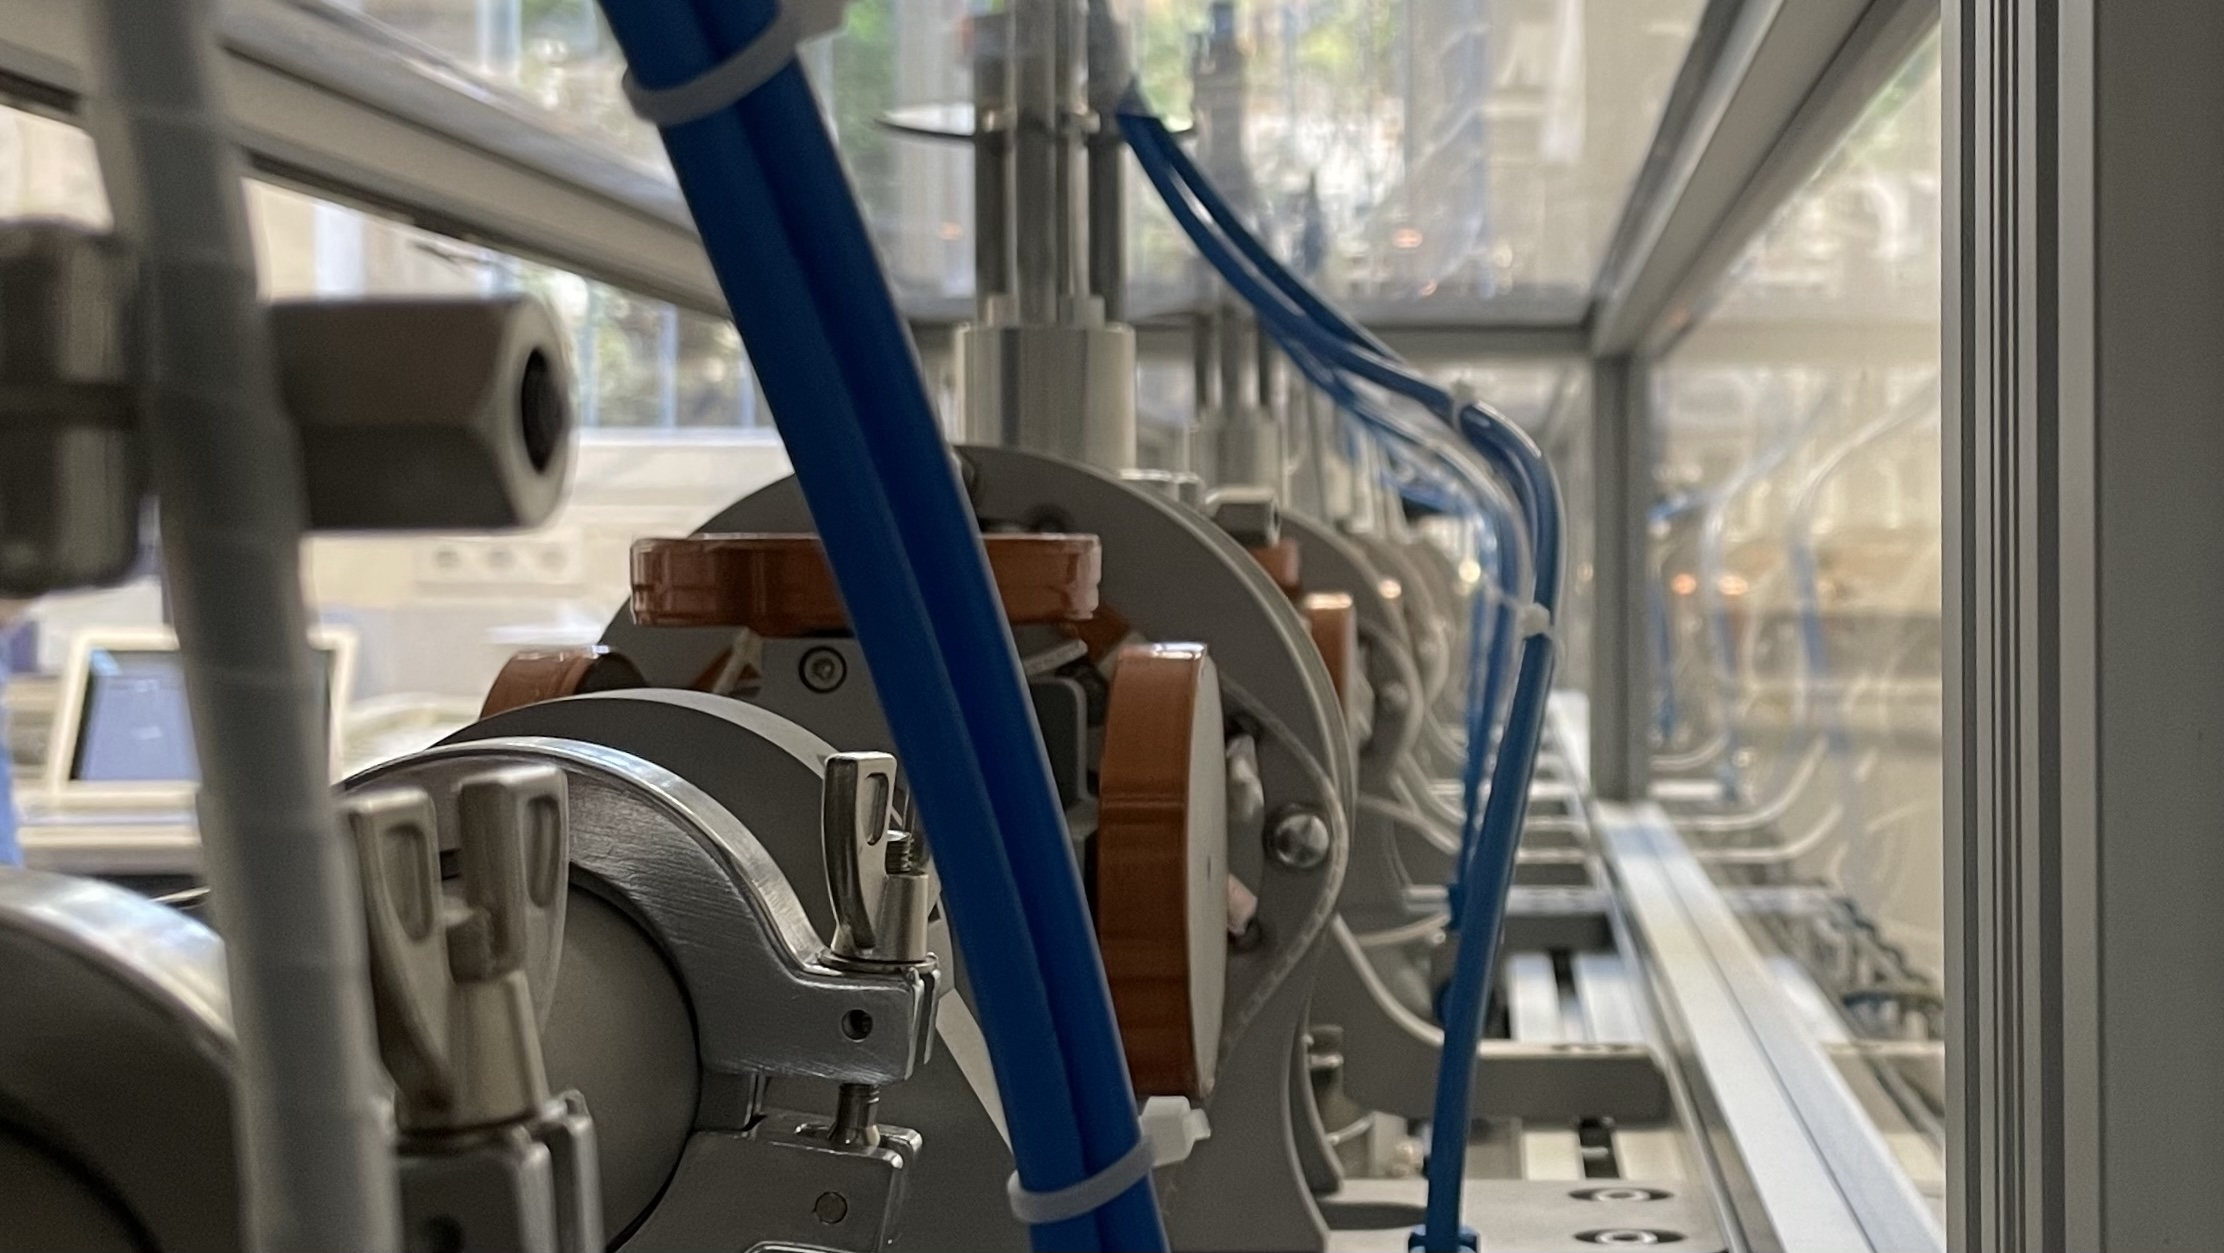
\includegraphics[width=\linewidth]{titlepic}
\vspace{-.2cm}

\rule{12cm}{1pt} \\\vspace{-.6cm} \rule{10cm}{1pt}
\end{center}

\renewcommand{\abstractnamefont}{\normalfont\scriptsize\bfseries}
\renewcommand{\abstracttextfont}{\normalfont\scriptsize}

\begin{abstract}
	In this report we determine the emittance of the provided linear accelerator LAB. The emittance is a crucial quantity when operating an accelerator because it connects beam width with divergence. We determine the emittance in two ways; \begin{itemize}
		\item Quadrupole scan: we measure the beam width as a function of the quadrupole strength of selected quadrupoles. Linear beam dynamics dictate a quadratic relation from which we can then determine the emittance by a fit
		\item Multiscreen method: we measure the beam width for fixed quadrupole strength(s) at various screens, yielding a linear equation system whose solutions determine again the emittance
	\end{itemize}
Both approaches will be compared in the end.
\end{abstract}
\begin{center}
	\rule{10cm}{1pt} \\\vspace{-.6cm} \rule{12cm}{1pt}
\end{center}

\setcounter{page}{-1}
\newpage

\tableofcontents
\thispagestyle{empty}
\newpage
\section{Introduction}
In this experiment we investigated the properties of a simple linear accelerator. Our goal is to measure the \emph{emittance} of the beam, an important parameter in accelerator physics as is motivated in section \ref{sec:theo}, where we will give the necessary theoretical background. The next section \ref{sec:exp} contains a detailed description of the used experimental setup. Having introduced theory and experimental setup we show our measurements and analysis in section \ref{sec:anal}; First we center the beam with corrector magnets using \emph{beam based alignment}. After this we measure the emittance via the \emph{multiscreen-method} and the \emph{quadropol-scan-method}. Finally we draw a conclusion in section \ref{sec:conc}. 


\section{Theory}
\label{sec:theo}
In the following we will give a short introduction to \emph{linear beam dynamics} which will be a crucial tool for our analysis. We will not motivate in detail why this is generally a good approach, more details are given for example in \cite{wille}. The structure of this section is oriented like in \cite{script}.
\subsection{Accelerator coordinates}
In accelerator physics it is customary to define a coordinate system which moves on the optimal particle trajectory $s$ and describes relative offsets from this trajectory in horizontal ($x$) and vertical ($z$) direction. Such a coordinate system is depicted in figure \ref{fig:coord}.

\begin{figure}[htbp]
	\centering
	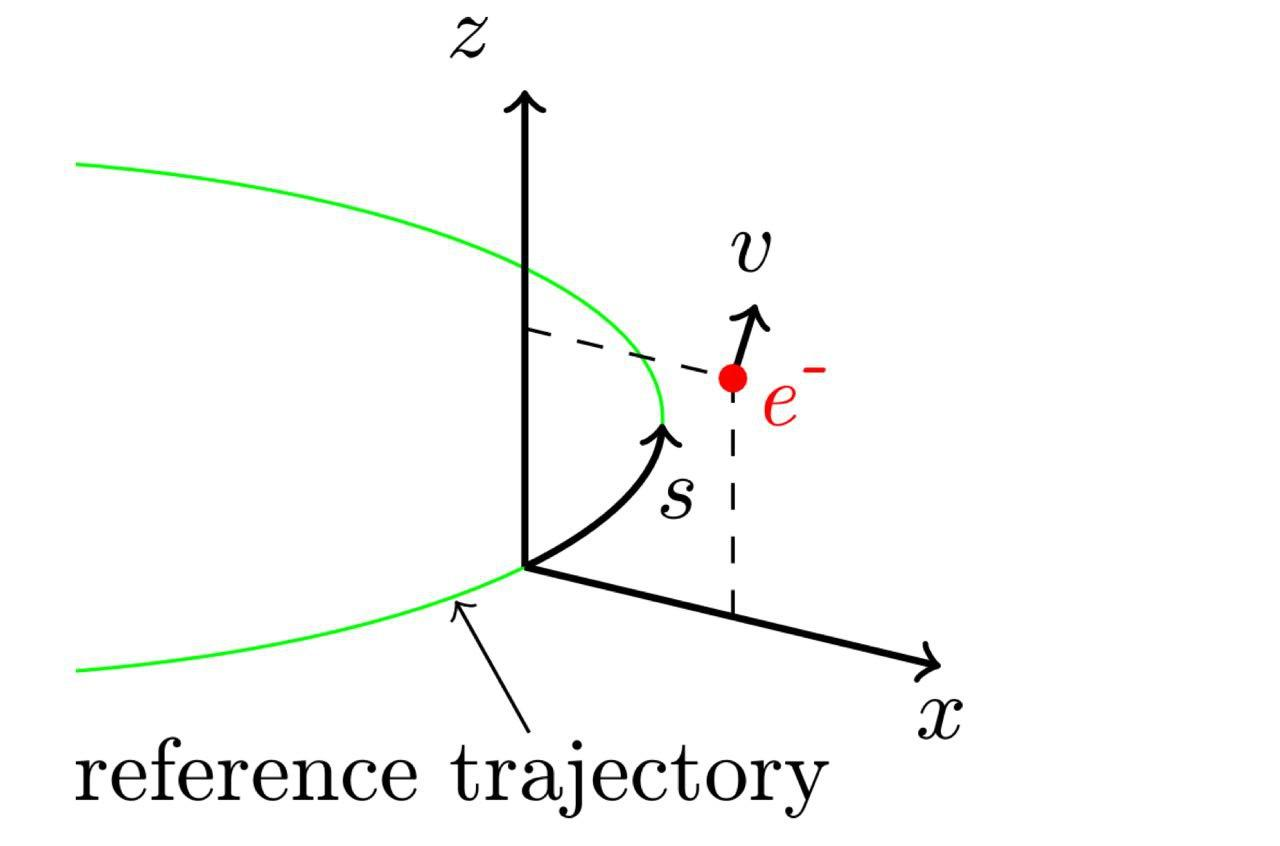
\includegraphics[width=.3\linewidth]{coord}
	\caption{Coordinate system around the optimal particle trajectory, taken from \cite{script}}
	\label{fig:coord}
\end{figure}

\subsection{\textsc{Hill}'s equations}
Particles do in general not solely follow the optimal trajectory but oscillate somewhat around it. This behavior is characterized by a set of differential equations, known as \textsc{Hill}'s equations \cite{wille}
\begin{align}
	x''(s)+\left(\frac{1}{R^2}(s)-k(s)\right)\cdot x(s)&=\frac{1}{R(s)}\frac{\Delta p}{p} \label{eq:hillx} \\
	z''(s)+k(s)\cdot z(s)&=0,
	\label{eq:hillz}
\end{align}
where $x'$ denotes the derivative with respect to the beam trajectory $s$. This means it denotes the angle to its optimal path in $x$ direction. $R(s)$ is the bending radius of any dipole magnet along the accelerator and $k(s)$ the quadropole strength. The fraction $\frac{\Delta p}{p}$ is the momentum spread which can often be neglected, especially in linear accelerators where $R(s)=\infty \forall s$. Since LAB is a linear accelerator both equations only differ by the sign of the quadropole strength $k(s)$ which indicates that a quadropole can only focus in one plane while it defocusses in the other plane, see section \ref{sec:exp}. A formal solution to equations \eqref{eq:hillx} and \eqref{eq:hillz} for an individual particle $i$ is given by $$\xi_i(s)=A_{\xi,i}\cos(\psi_\xi(s)+\phi_{\xi,i}),$$ with $\xi\in \{x,z\}$. 
Here $A_{\xi,i}$ is the particles individual amplitude and $\psi_\xi(s)$ and $\phi_{\xi,i}$ describe the particles phase advance and initial phase respectively \cite{wille}. 
\subsection{Matrix formalism}\label{subsec:Matrix_formalism}
Because of their linear form it is possible to write the propagation through different elements of the accelerator analogous to matrix optics. The properties of interest are the displacement and angle in $x,z$ direction.

 \begin{equation}
 	\begin{pmatrix}
 		\vec{x}(s_1) \\ \vec{z}(s_1)
 	\end{pmatrix}
 =\begin{pmatrix}
 	M_x  & 0 \\
 	0 & M_z
 \end{pmatrix}
\cdot
\begin{pmatrix}
	\vec{x}(s_0) \\ \vec{z}(s_0)
\end{pmatrix}
\end{equation}
Here $M_{\xi}\in2 \times 2$ are two dimensional quadratic matrices with determinant 1 and the vector $\vec{\xi}=(\xi,\xi')^T, \xi\in\{x,z\}$ \cite{wille}. In the following the matrices for the needed optical elements of LAB will be given without derivation, see for example \cite{wille}.
\subsubsection*{Drift}
A drift of length L can be represented by
\begin{equation}
	M_{\text{drift}}=\begin{pmatrix}
		1 & L & 0&0\\
		0 & 1 & 0&0\\
		0&0&1&L\\
		0&0&0&1
	\end{pmatrix}.
\end{equation}

\subsubsection*{Quadrupoles}
When looking at quadrupoles we have to distinguish between focusing (QF) and defocusing (QD) quadrupoles with respect to the horizontal plane\footnote{This choice is arbitrary one could also choose to define focus and defocus with respect to the vertical plane}. Here an approximation is already made (thin lense approximation). With the quadropole strength $k$ and length $L$ we find 
\begin{align}
	M_{\text{QF}}=\begin{pmatrix}
		1 & 0 & 0&0\\
		-kL & 1 & 0&0\\
		0&0&1&0\\
		0&0&kL&1
	\end{pmatrix}
&&
	M_{\text{QD}}=\begin{pmatrix}
	1 & 0 & 0&0\\
	kL & 1 & 0&0\\
	0&0&1&0\\
	0&0&-kL&1
\end{pmatrix}.
\end{align}
\subsubsection*{Corrector Magnets}
Corrector magnets cannot be represented by a matrix multiplication and will be treated like drifts of the length of the corrector \cite{script}.
\subsubsection*{Transfer matrix of multiple elements}
Like in optics the passing through several elements can be accounted for by simply multiplying the respective matrices. For example the propagation \begin{center}
	$\to$QF$\to$drift$\to$QD$\to$
\end{center} will be given by 
\begin{equation}
		M_{\text{total}}=M_\text{QD}\cdot M_\text{drift}\cdot M_\text{QF}.
\end{equation}



\subsection{Phase space, emittance and twiss parameters}
The beam consists of many particles with individual trajectories $\xi_i(s)$ and amplitudes $A_{\xi,i}(s)$ whose distribution delivers the profile of overall beam, see figure \ref{fig:beam}.
\begin{figure}[htbp]
	\centering
	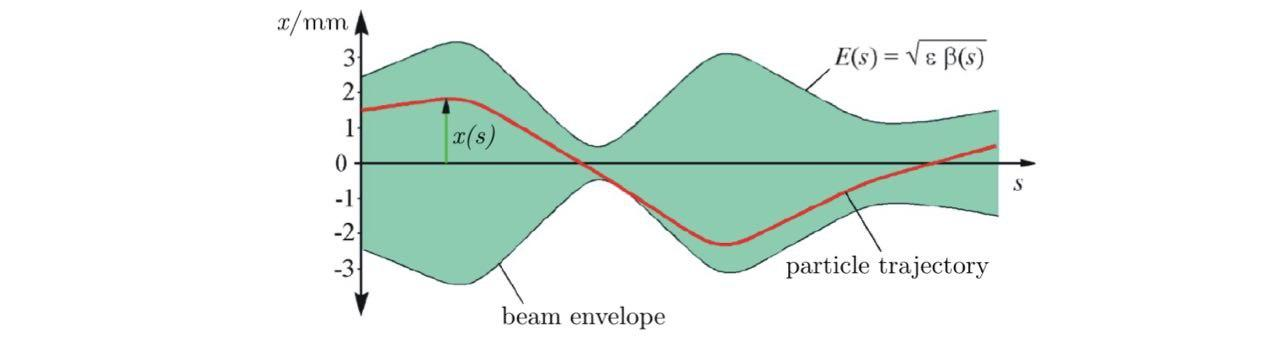
\includegraphics[width=.7\linewidth]{beam}
	\caption{Beam envelope consisting of the many individual particle trajectories, taken from \cite{script}}
	\label{fig:beam}
\end{figure} 
The envelope is then given by the amplitude of a particle at $1\sigma$ of this distribution \cite{script} and can be written as 
\begin{equation}
	E(s)=\sqrt{\epsilon\cdot\beta(s)},
\end{equation}
with the \emph{emittance} $\epsilon$ and the \emph{beta function} $\beta(s)$. The emittance is a measure of the ability to focus the beam and the beta function describes how the optical elements influence the beam profile \cite{script}. The emittance is a conserved quantity. In phase space of the coordinates $\xi,\xi'$ they describe an ellipse whose area is given by the emittance. Part of the ellipse equation are the so called \emph{Twiss} parameters $\alpha,\beta,\gamma$ (see figure \ref{fig:ellipse}).

\begin{figure}[htbp]
	\centering
	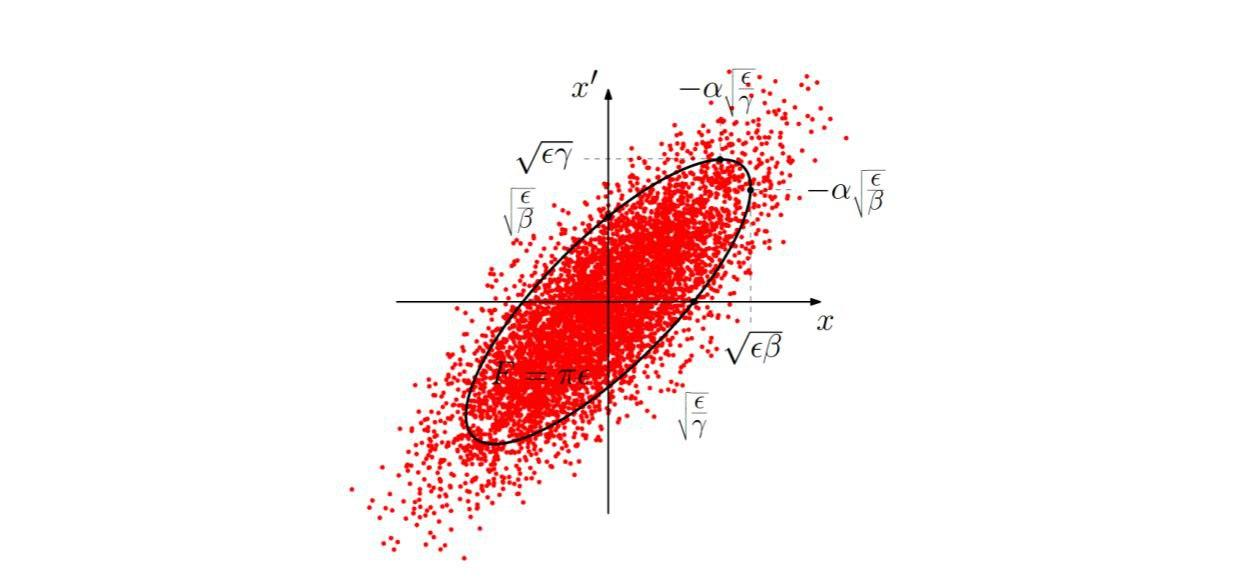
\includegraphics[width=.7\linewidth]{ellipse}
	\caption{ellipse in horizontal phase space taken from \cite{script}}
	\label{fig:ellipse}
\end{figure}

 While $\alpha(s)$ is a measure for the correlation between $\xi(s)$ and $\xi'(s)$, $\beta(s)$ and $\gamma(s)$ are a measure of beam width $\sigma_\xi=\sqrt{\epsilon\beta(s)}$ and angular width $\sigma_{\xi'}=\sqrt{\epsilon\gamma(s)}$ respectively \cite{script}. The Twiss parameters can also be described with the matrix formalism. For this we define the Beta matrix \begin{equation}
	B_\xi(s):=\begin{pmatrix}
		\beta_\xi(s) & -\alpha_\xi(s)\\
		-\alpha_\xi(s)& \gamma_\xi(s)
	\end{pmatrix}
\end{equation}
which propagates from point $s_0$ to $s_1$ as \cite{wille}

\begin{equation}
	\label{eq:beta}
	B_\xi(s_1)=M_\xi\cdot B_\xi(s_0)\cdot M_\xi^T.
\end{equation}


\newpage
\section{Experimental Setup}
\label{sec:exp}
In this section we will explain the principle of operation for the 3m long electron LAB accelerator. A principle schematic is given by figure \ref{fig:experimental_setup}. The accelerator consist of the following components. All informations were taken from \cite{script}. 
\begin{figure}[h]
	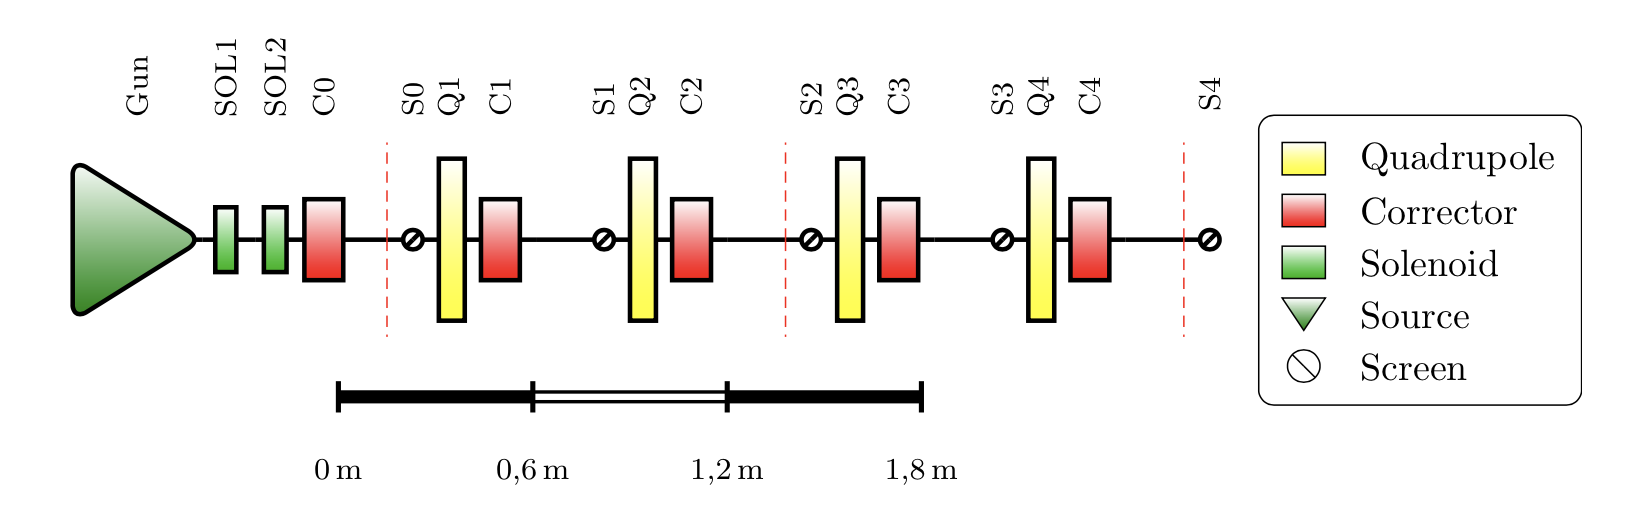
\includegraphics[width=\linewidth]{./figs/experimental_setup.png}
	\caption{Principle schematic of the LAB accelerator \cite{script}}\label{fig:experimental_setup}
	\label{fig:aufbau}
\end{figure}

\subsection{Electron gun}
The electron gun creates the electron beam by accelerating free electrons from a heating wire to about $0.3c$. In a heating wire (or filament) electrons get high kinetic energies and overcome the work function of the material (thermionic emission). The heating wire is encased by the cathode. Between both of them lies a small potential difference (10V-180V) so that the electrons get accelerated in direction of the cathode. A \textsc{Wehnelt} cylinder can be used as a focusing element but isn't used in the actual experiment, since it doesn't have a significant influence. Between the anode (ground) and the cathode lies a potential difference of about $-25$keV. The electrons are accelerated by the electric force and reach a velocity of $0.3c$, for which relativistic effects can be neglected. Because electrons build up space charge zones an electron beam naturally diverges. To counter this effect the cathode and anode  have special shapes to create a focusing electric field. The cathode has a tapered outer shape with the so called \emph{Pearce} angle while the anode matches this shape. The electron beam leaves the cathode a $0.5$ mm hole at an emission current of a few $\mu$A and reaches accelerated a $10$mm hole in the anode. This type of electron gun is also called a \emph{inverted} gun. Only this element defines the beam quality and therefore the emittance $\epsilon$. A principle schematic of the electron gun is given in figure \ref{fig:gun}.

\begin{figure}
	\centering
	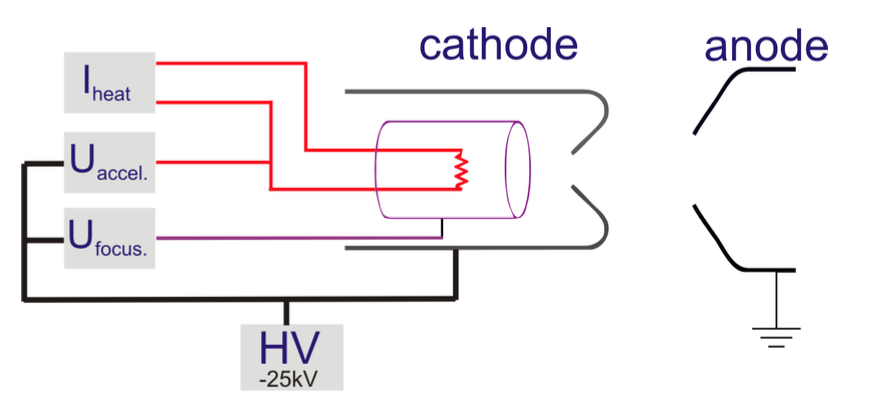
\includegraphics[width=0.6\linewidth]{figs/electron_gun.png}
	\caption{Principle schematic of the inverted electron gun \cite{script}}\label{fig:gun}
\end{figure}
\subsection{Solenoids}
The accelerated electrons first off all pass through two solenoid magnets. They are aligned parallel to the beam axis $s$, as their magnetic fields. If electrons have transversal momentum components the \textsc{Lorentz} force applies and the trajectory gets bent. This has a focusing effect on the beam.
\newpage
\subsection{Corrector Magnets}
\begin{wrapfigure}{r}{0.35\textwidth}
	\vspace{-1cm}
	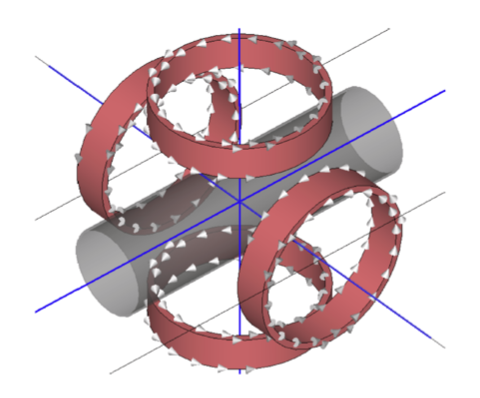
\includegraphics[width=\linewidth]{figs/corrector_magnets.png}
	\caption{Corrector magnet \cite{script}}\label{fig:corrector_magnets}
\end{wrapfigure}
The corrector magnets deflect the beam horizontally and/or vertically. Even if the beam comes in a perfect angle relative to the optical elements, influences like the magnetic field of earth have to be compensated for this relatively slow velocities. The trajectory of an incoming electron beam gets bend by two opposite coils in an almost \textsc{Helmholtz} configuration. In such a homogeneous magnetic field, the bending angle $\alpha$ (or \emph{kick}) follows from the \textsc{Lorentz} force  and the small angle approximation as 
$$\alpha=\frac{e\cdot B\cdot L}{p}$$ with the electron charge $e$,the magnetic field $B$ and where $L$ denotes the effective length of the magnet.

Because the magnetic field doesn't end at the ends of a magnet and rather decreases continuously, the field length does not equal to the physical length of the magnet. Therefor the effective length describes the hypothetical length of a constant field $B_\text{max}$. Figure \ref{fig:effective_length} depicts the effective length of a homogeneous field with continuously decreasing edges. In the experiment the corrector magnet configuration is used as shown in figure \ref{fig:corrector_magnets}. By using superposition a trajectory bend can be done in the $x$- and $z$-axis simultaneously.

\begin{figure}[h]
	\centering
	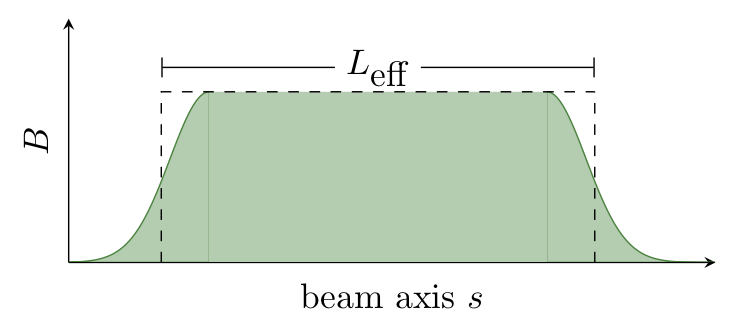
\includegraphics[width=0.5\linewidth]{figs/effective_length.png}
	\caption{Sketch of a homogeneous magnetic field and the effective length $L_\text{eff}$ \cite{script}}\label{fig:effective_length}
\end{figure}
\newpage
\subsection{Quadrupole magnets}
\begin{wrapfigure}{r}{0.35\textwidth}
	\vspace{-.8cm}
	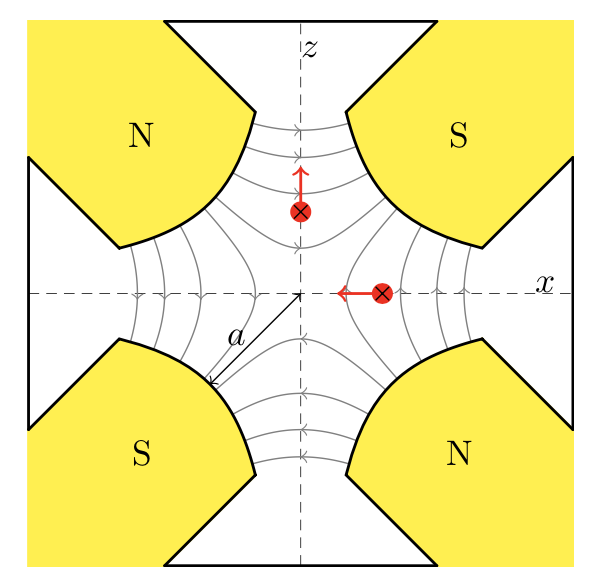
\includegraphics[width=\linewidth]{figs/quadrupole.png}
	\caption{Quadrupole magnet in beam plane \cite{script}}\label{fig:quadrupoles}
\end{wrapfigure}
Quadrupole magnets (short quadrupoles) are focusing elements for particle beams. They consist of four magnets with altering polarizations as depicted in figure \ref{fig:quadrupoles}. At the center of the quadrupole aren't any magnetic fields and therefor no deflections. Only charged particles that cross the quadrupole magnet with a slight offset to the ideal beam line experience the \textsc{Lorentz} force. Since magnetic field lines go from north to south poles a deflection happens either to the center or the outside depending on the electron position in the quadrupole (compare \ref{fig:quadrupoles}). A quadrupole can for this fact, only be focusing in one axis, while being defocusing in the other. This is a big difference to optical lenses. One can find this effect in equations \ref{eq:hillx} and \ref{eq:hillz}, where the signs alter. To get an overall focusing system, one has to set an inverted quadrupole in the focal length $$f=\frac{1}{kL}.$$
The quantity $k$ is the so called quadrupol strength that is defined by the electron charge $e$, electron momentum $p$ and the gradient of the electric field $g$:
$$k=\frac{e}{p}\cdot g = \frac{e}{p}\frac{\partial B_z}{\partial x}= \frac{e}{p}\frac{\partial B_x}{\partial z}$$
If the beam does not enter the quadrupole centered, a kick will apply to the beam as by the corrector magnets. This property will be used to do the beam alignment.


\subsection{Screens}

\begin{wrapfigure}[10]{r}{0.3\textwidth}
	\vspace{-2.5cm}
	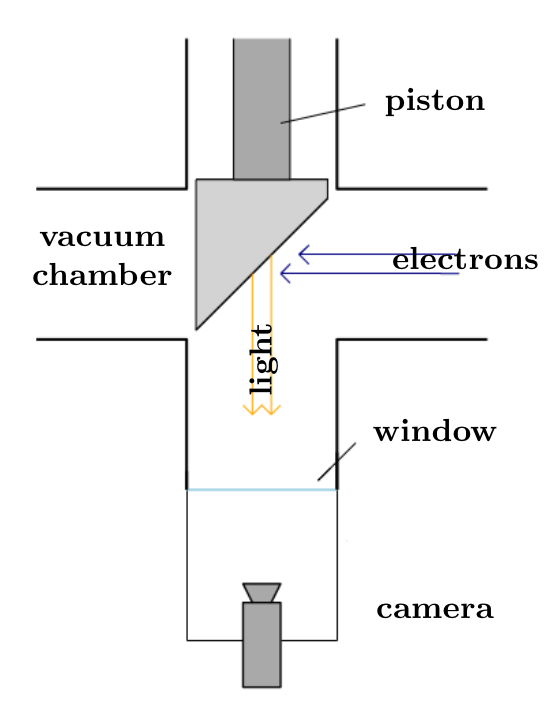
\includegraphics[width=1\linewidth]{figs/screen.png}
	\caption{Principle schematic of the Screen \cite{script}}\label{fig:screens}
\end{wrapfigure}

To calibrate and visualize the beam, one can insert a screen in the beam line. The screen is angled $45^\circ$ to the beam axis and is made of fluorescent aluminium oxide. The $45^\circ$ angle delivers a $1:1$ depiction of the electron beam. The interaction of the electrons with the screen result in the creation of photons, that can be captured by a camera with lens. The screen is destructive to the beam. Only a few electrons can penetrate through the screen and get deflected by scattering processes. The screens get placed with air pressure without destroying the vacuum in the tube. 
\subsection{Composition}
As depicted in figure \ref{fig:experimental_setup} the first element after the electron beam are two solenoid magnets (SOL1/2), followed by the first corrector magnet (C0) and screen (S0). After that four times a combination of a quadrupole magnet, a corrector and a screen follows. Different from the illustration, the length between the quadrupole and corrector magnets is far bigger. If it wouldn't be, then a proper beam alignment wouldn't be possible, since the \emph{kick} of the quadrupole to an unaligned beam couldn't be seen. The electron gun and all optical elements are placed in a vacuum to suppress particle scattering. In table \ref{tab:LAB_properties} are properties of the corrector and quadrupole magnets listed. Table \ref{tab:LAB_dimensions} provides informations about lengths of the accelerator, which are needed for later calculations.
\begin{table}[]
	\centering
	\begin{tabular}{|l|l|l|}
		\hline
		Paramers                         & Corrector         & Quadrupole         \\
		\hline
		coil geometry                    & round             & rectangular        \\
		coil radius                      & $40$mm            & 52mm $\times$ 72mm \\
		number of windings               & 300 (in 8 layers) & 120 (in 4 layers)  \\
		coil distance                    & 105 mm            & 28 mm              \\
		wire diameter                    & 0.3 mm            & 0.3 mm             \\
		physical length $L_\text{phys.}$ & 80 mm             & $(71.3\pm0.5)$ mm  \\
		effective length $L_\text{eff.}$ & 78.5 mm           & $(74\pm1)$mm      \\
		\hline
	\end{tabular}
	\caption{Properties of the corrector and quadrupole magnets \cite{script}}\label{tab:LAB_properties}
\end{table}
\subsection{Measurement and control software}
We can steer every part of the accelerator via a GUI (LAB control system) on a computer in the lab room. Measurements of the position and width are performed by software which fits a two dimensional \textsc{Gaussian} to the beam profile in a selected area. 

\section{Measurements and Analysis}
In this section we will verify the applied calibration to the corrector magnets and proceed to a beam-based alignment. Afterwards we measure the emittance by two methods, namely the quadrupole scan and Multiscreen-method. At the end of this section we will briefly discuss the influences of systematic errors.
\label{sec:anal}
\subsection{Verification of the calibration}
Before starting any measurements or doing the beam alignment we will verify the linear relation between the kick angle $\alpha_{x,z}$ and the position on the screen. For this we chose the correctors C0 and C1 with the associated screens S0 and S1. The quadrupole Q1 was shut down for this verification. We then measured the relative position of the beam center in dependence on the kick angle $\alpha$. This was done for the $x$- as well as the $z$-axis. The results are depicted in figure \ref{fig:kick_verify}.
\begin{figure}[h]
	\centering
	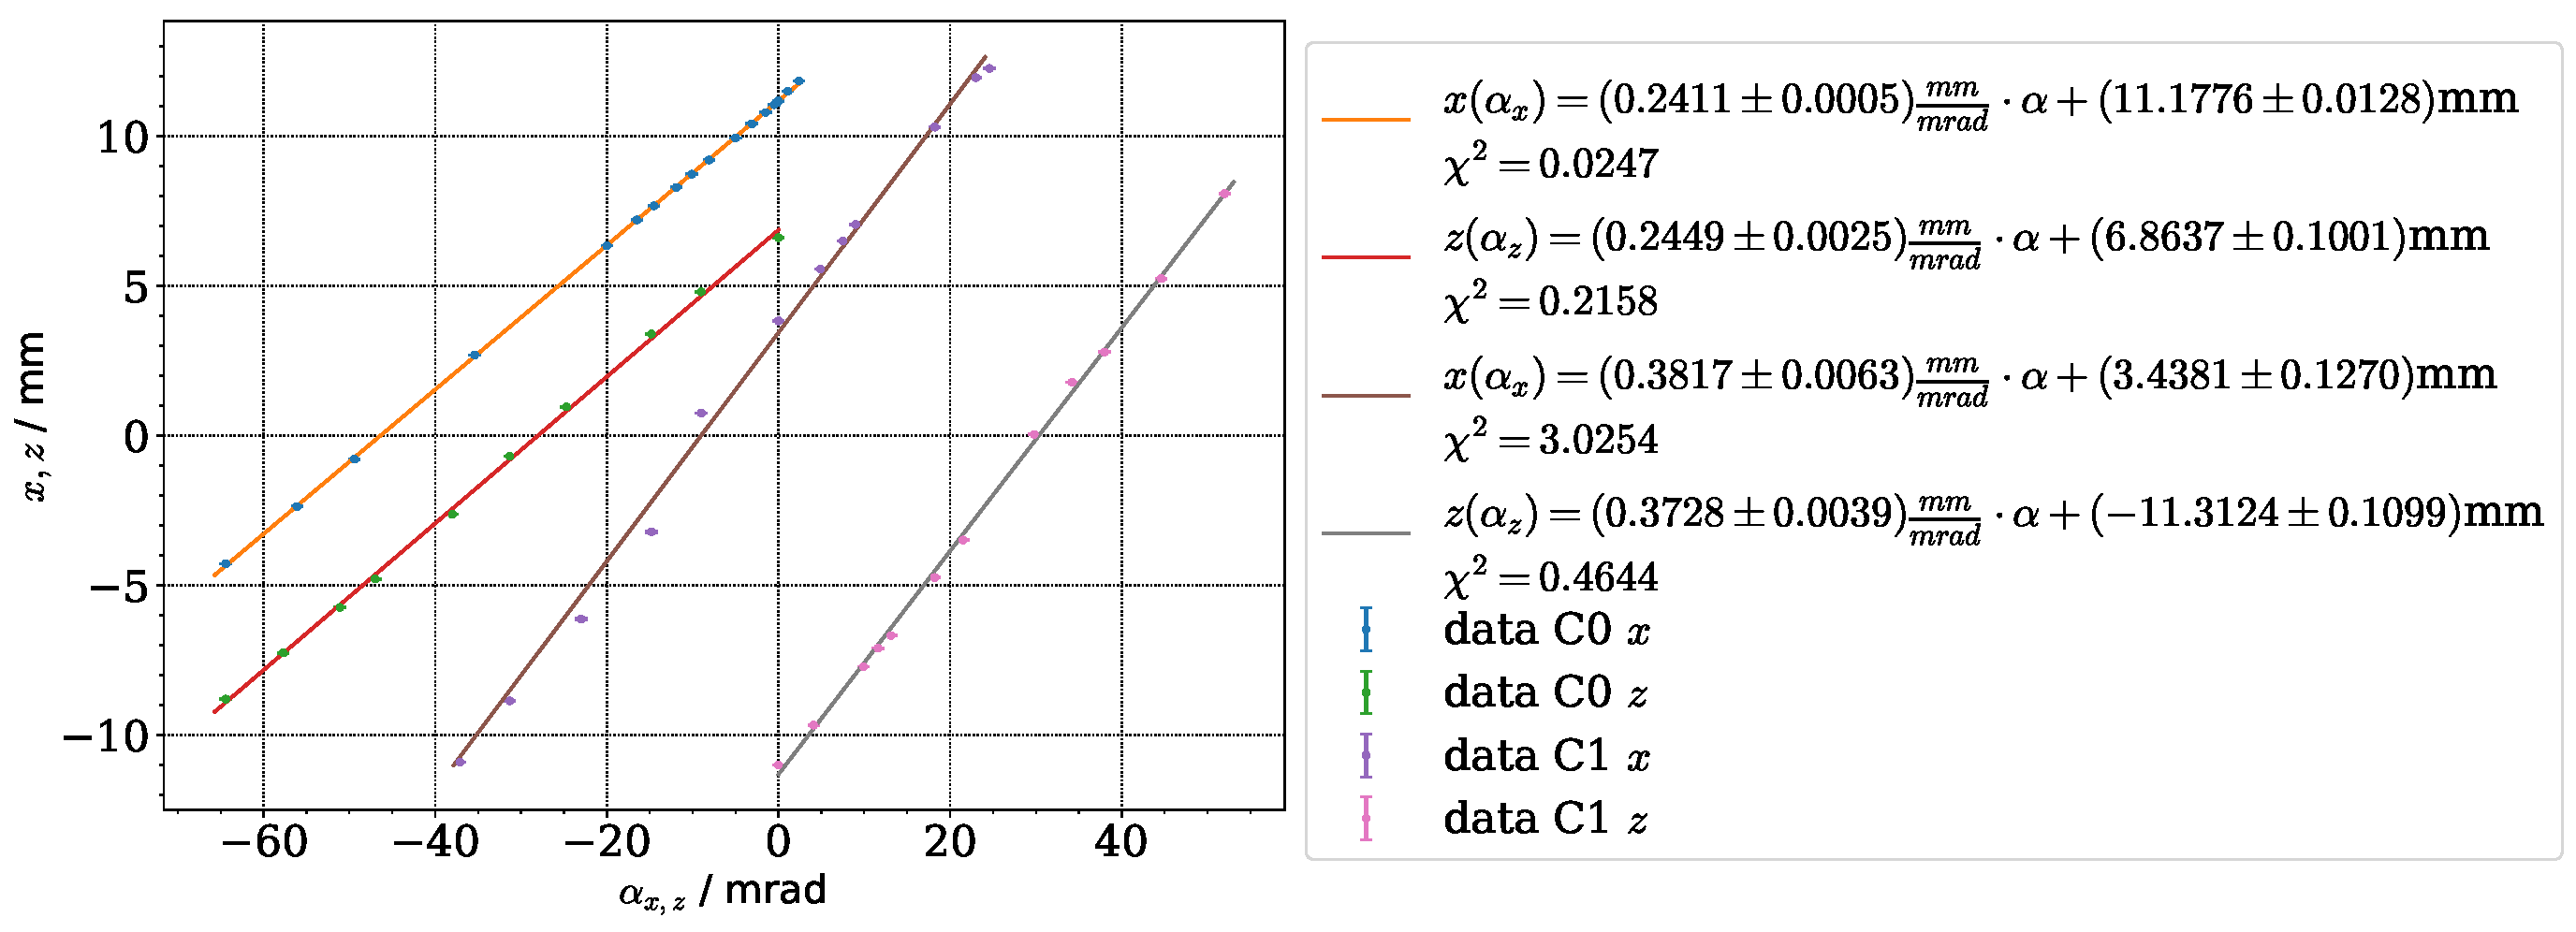
\includegraphics[width=\linewidth]{figs/calibration/kick_verification.pdf}
	\caption{Verification of linear relation between the kick angle $\alpha$ and the offset $x$, $z$}\label{fig:kick_verify}
\end{figure}

For both corrector magnets follows a linear relation between the kick angle $\alpha$ and the screen position. This relation can be written for small angles $x'$ and $z'$ as 
\begin{align*}
	\alpha_x\approx \sin(\alpha_x)=\frac{\Delta x}{L} && \text{ and } && \alpha_z\approx \sin(\alpha_z)=\frac{\Delta z}{L}
\end{align*}
with the drift length $L$. The offsets seen in figure \ref{fig:kick_verify} are arbitrary since those are just relative positions and not related to the real screen center or ideal beam center at all. 
With the small angular approximation one can write the drift length $L$ as the derivatives
$$\frac{\partial x}{\partial \alpha_x}=\frac{\partial z}{\partial \alpha_z}=L$$

We compare our slopes of figure \ref{fig:kick_verify} with the given drift lengths from the LAB manual \cite{script} (compare table  \ref{tab:LAB_dimensions}) in table \ref{tab:verify} and find that they differ by more than one standard deviation. This result shall be fine, since we used the effective lengths rather then the physical lengths. The applied kick is also not instantaneous.  In appendix \ref{sec:additional_verficitation} we inspected the linear relation between the applied current against the offset $x$ and $z$. Overall one can say, that the calibration is good enough and we can proceed.
\begin{table}
	\centering
	\begin{tabular}{|c|c|c|c|}
		\hline
		Screen &$\frac{\partial x}{\partial \alpha_x}$ / m  &$\frac{\partial z}{\partial \alpha_z}$ / m  & $L$ / m\\
		\hline
		S0 & $0.2411\pm 0.0005$ & $0.2449\pm 0.0025$ & 0.2635 \\
		S1 &$0.3817\pm 0.0063$&$0.3728\pm 0.0039$& 0.3945\\
		\hline
	\end{tabular}
	\caption{Drift lengths -- calculated and manual values \cite{script}}\label{tab:verify}
\end{table}

\subsection{Beam-based alignment}
For every particle accelerator experiment a proper aligned beam is necessary. To align the beam we will use the corrector and quadrupole magnets. Only if the particle beam goes straight through the center of the quadrupole, no deflection (quadrupole kicks) happen. The quadrupole therefor should only have influence on the beam focus and not on the position. We will align the beam by passing it through a quadrupole that switches between two quadrupole strengths $k\in\{-30,30\}\frac{1}{\text{m}^2}$. If the position of the beam profile on the following screen doesn't change, the beam is properly aligned. This was first done by eye. 

After the first alignment we followed the recipe from the script \cite{script}:
\begin{enumerate}
	\item The kick  (current $I_x^C$) of a corrector magnet in front of the quadrupole is used to set the position where the beam passes the quadrupole.
	\item The strength (current) of the quadrupole is varied by a fixed value $\Delta k$ ($\Delta I^Q$).
	\item The resulting beam displacement $\Delta x$ is measured on a screen behind the quadrupole.
	\item Do a linear fit and find the zero point.
\end{enumerate}

Figure \ref{fig:quad_calib_1} depicts the beam alignment for the first corrector (C0) by using the quadrupole (Q1). One can find the other linear fits in the appendix \ref{fig:quad_calib_rest}. Table \ref{tab:kick_settings} lists all found ideal kick angles $a_\text{ideal}$. We also listed the set values $\alpha_\text{set}$ because one couldn't set all values that we found in the control software. We also didn't specify an error in this table, because we set the values fixed in the software after this determination. Another argument is, that we did the error analysis later and not at the lab itself. All calculated errors can be found at the associated plots. Overall follows that if the alignment isn't proper all other results will be influenced systematically. This error can't be removed after the lab session and for this the choice of the kick was final. 

The settings of the last corrector C4 are mentioned in table \ref{tab:kick_settings}, but since it wasn't calibrated -- because it only serves the purpose of centering the beam on the last screen -- one can set the parameters as wanted.

\begin{figure}
	\begin{subfigure}{.49\linewidth}
		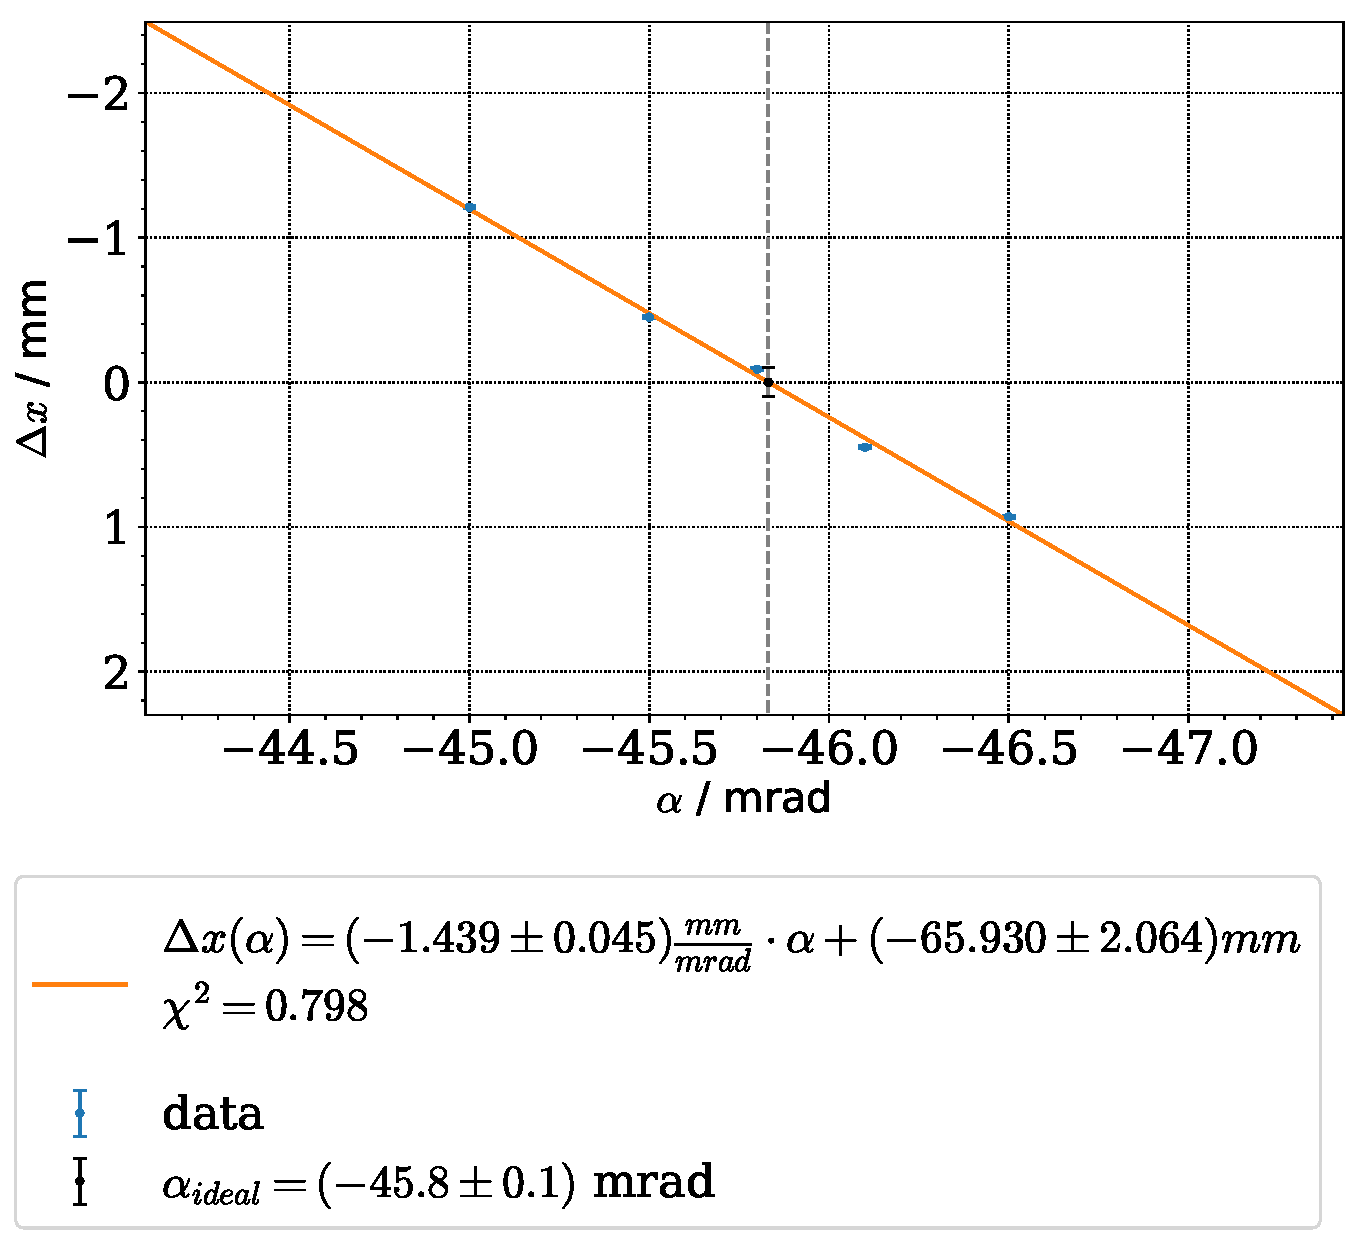
\includegraphics[width=\linewidth]{figs/calibration/q1_x.pdf}
		\caption{$x$-axis}
	\end{subfigure}
	\begin{subfigure}{.49\linewidth}
		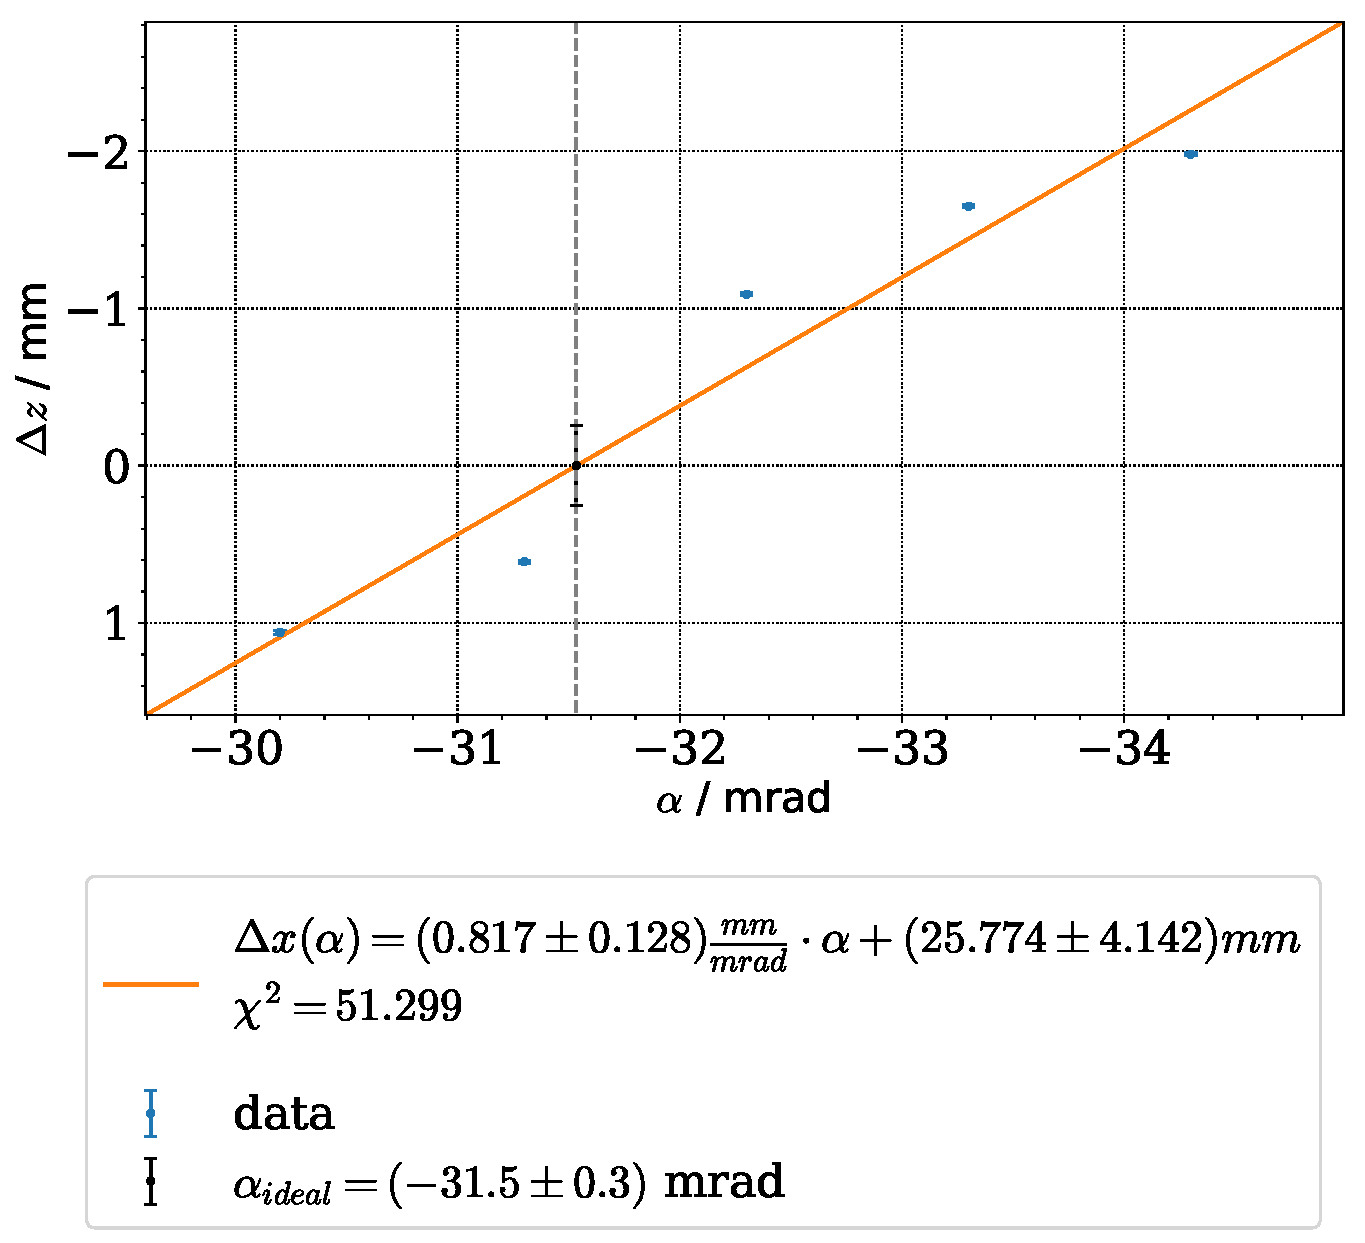
\includegraphics[width=\linewidth]{figs/calibration/q1_z.pdf}
		\caption{$z$-axis}
	\end{subfigure}
	\caption{Beam alignment in the $x$- and $z$-axis for the corrector C0}\label{fig:quad_calib_1}
\end{figure}

\begin{table}[H]
	\centering
	\begin{tabular}{|c|c|c|c|c|}
		\hline
		Corrector&$\alpha^x_\text{ideal}$ / mrad &$\alpha^z_\text{ideal}$ / mrad &$\alpha^x_\text{set}$ / mrad &$\alpha^z_\text{set}$ / mrad  \\
		\hline
		C0&  -45.8 & -31.5&-45.8&-31.6\\
		C1& -10.7& 26.8 &-10.8&26.9\\
		C2&  -31.8 & 10.9&-31.9&11.0\\
		C3& -29.2& 15.4 &-29.3&15.4\\
		C4 &--&--&-31.9&18.9\\
		\hline
	\end{tabular}
	\caption{kick settings for the corrector magnets}\label{tab:kick_settings}
\end{table}
\subsection{Beam transport}
To our surprise the ideal values $\alpha_\text{ideal}$ almost matched the ones we set before by eye. In figure \ref{fig:Screenshots} are screenshots of our calibrated and eyeballed beam depicted. To reproduce the beam profile from the first screen at the last screen we employed alternating quadropole strengths of $k_Q=\pm\SI{30}{m^{-2}}$ in the four quadrupoles. The second screen S1 as seen in figure \ref{fig:ScreenS1} is damaged and distorts the image of the beam. Since the beam looks undistorted on the following screens, it can be said, that it's the fault of the screen and not of the optical elements. Screen S4 --depicted in figure \ref{fig:ScreenS4}-- shows also a distorted beam profile. This is the result of magnetic fields produces by the operation and measurement electronics, that are placed directly behind the screen. Generally we can say that we were able to reproduce the beam profile from the start to the end. The last screen is not really a reliable indicator of beam quality as said before. But up to screen 3 we can keep the beam focused and aligned well which we can conclude from the high beam intensity in a small area. We can also clearly see the focusing power of quadropules in action. While we start as a almost circular "blob" at screen 1 the beam profile is focused in horizontal/vertical direction and smeared out in vertical/horizontal direction. After the next quadrupole we return to our circular blob and repeat the process. The aligned beam is able to reproduce a high intensity blob already after the first two quadrupoles which is not performed by the alignment by eye. This is a good sign our alignment went well.    
\begin{figure}[htbp]
	\begin{subfigure}{0.19\linewidth}
		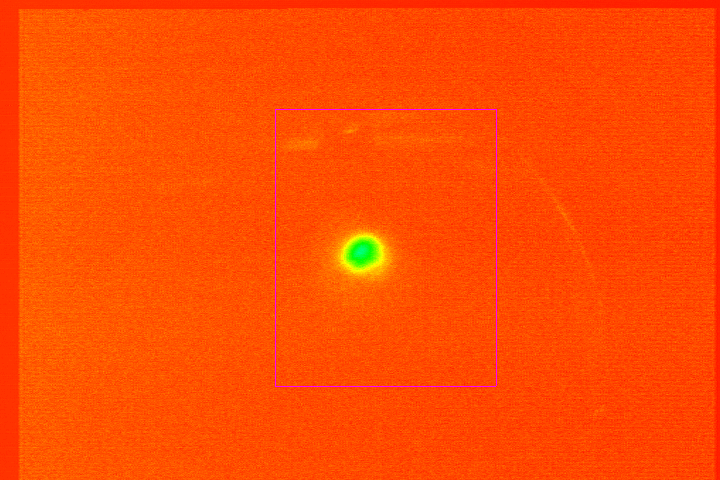
\includegraphics[width=\linewidth]{figs/Screens/S0_Eyeball.png}
		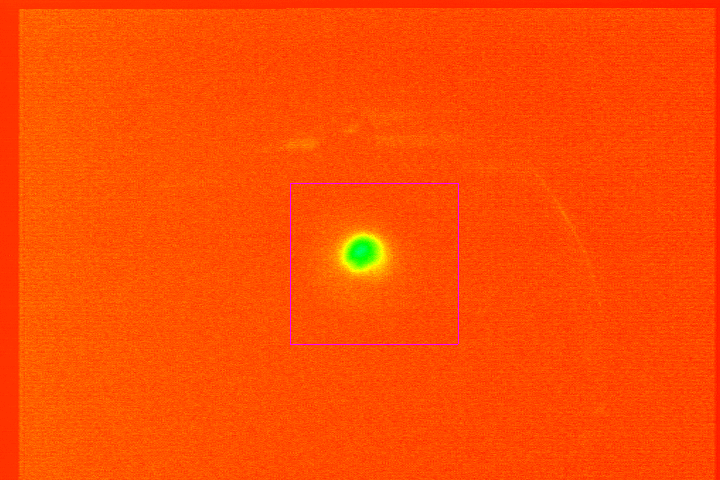
\includegraphics[width=\linewidth]{figs/Screens/S0_Calib.png}
		\caption{Screen S0}
	\end{subfigure}	\hfill
	\begin{subfigure}{0.19\linewidth}
		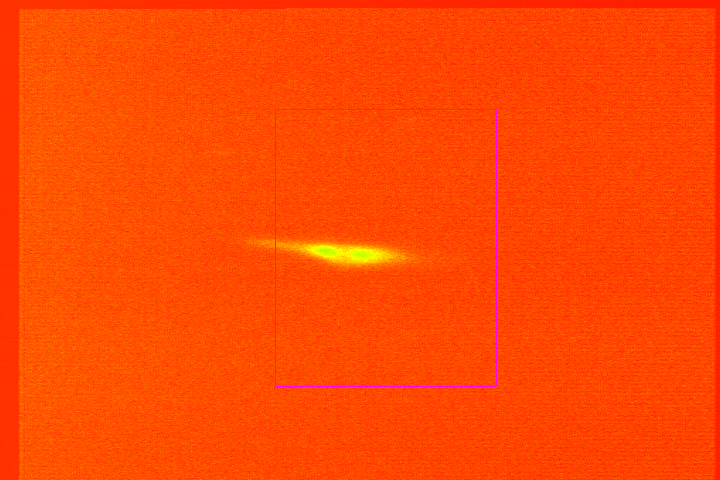
\includegraphics[width=\linewidth]{figs/Screens/S1_Eyeball.png}
		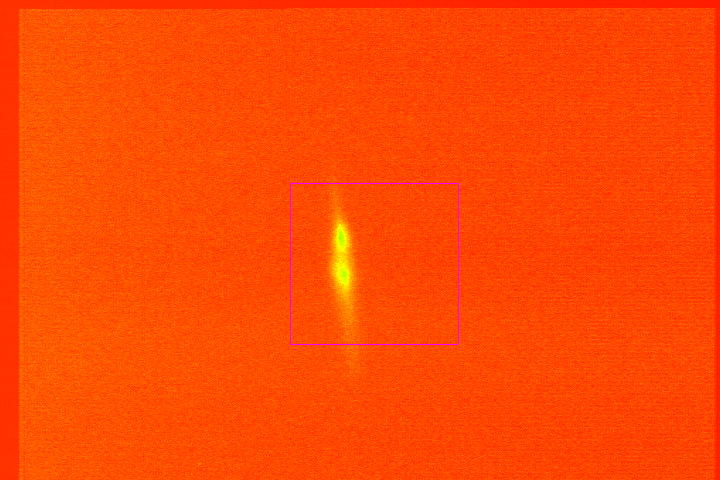
\includegraphics[width=\linewidth]{figs/Screens/S1_Calib.png}
	\caption{Screen S1}\label{fig:ScreenS1}
	\end{subfigure}	\hfill
	\begin{subfigure}{0.19\linewidth}
		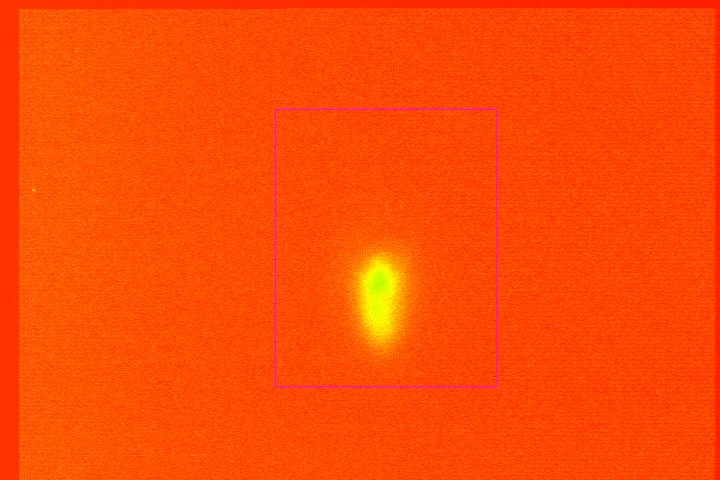
\includegraphics[width=\linewidth]{figs/Screens/S2_Eyeball.png}
		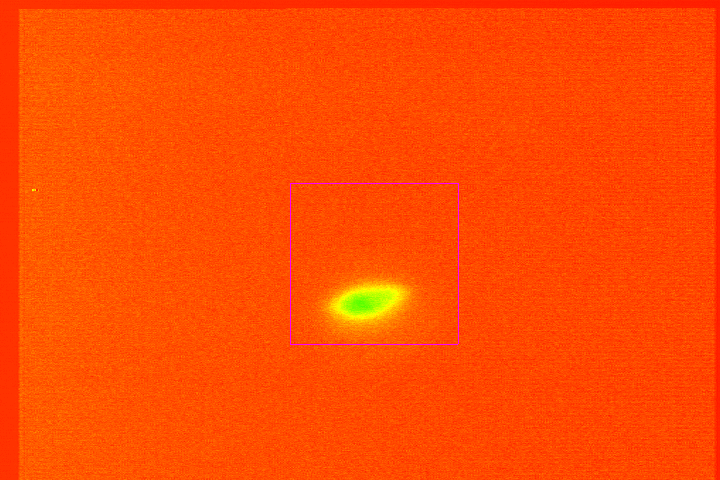
\includegraphics[width=\linewidth]{figs/Screens/S2_Calib.png}
		\caption{Screen S2}
	\end{subfigure}	\hfill
	\begin{subfigure}{0.19\linewidth}
		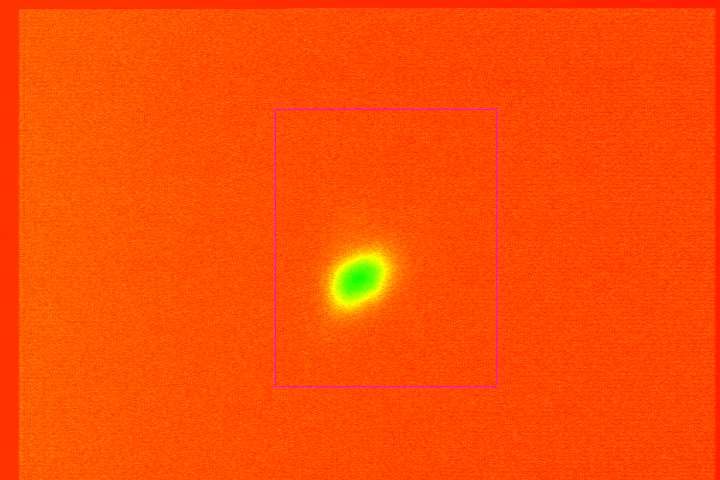
\includegraphics[width=\linewidth]{figs/Screens/S3_Eyeball.png}
		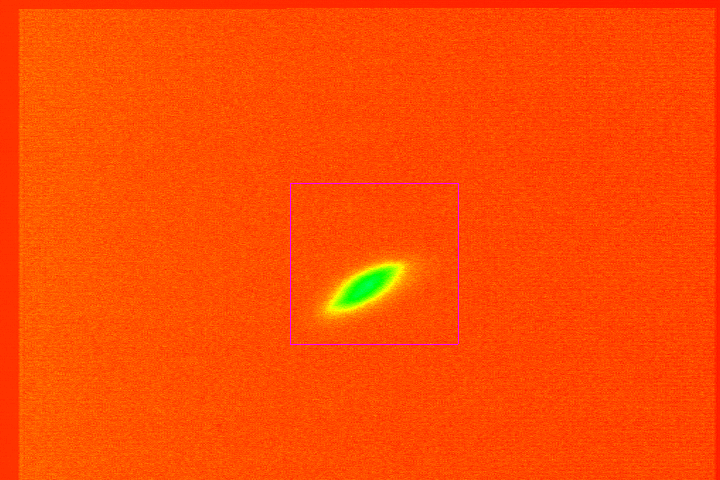
\includegraphics[width=\linewidth]{figs/Screens/S3_Calib.png}
		\caption{Screen S3}
	\end{subfigure}	\hfill
	\begin{subfigure}{0.19\linewidth}
		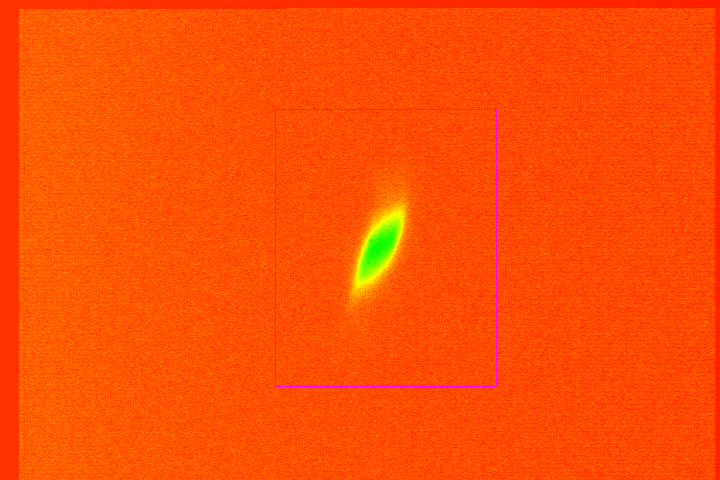
\includegraphics[width=\linewidth]{figs/Screens/S4_Eyeball.png}
		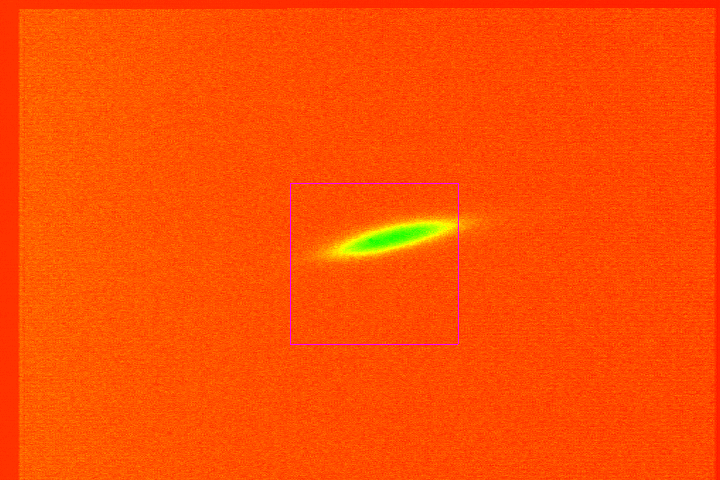
\includegraphics[width=\linewidth]{figs/Screens/S4_Calib.png}
		\caption{Screen S4}\label{fig:ScreenS4}
	\end{subfigure}	
	\caption{Screen shots of the beam. Upper row aligned by eye and lower row aligned by beam-based alignment. The beam intensity ranges from low (red) to high (green).}\label{fig:Screenshots}
\end{figure}
\subsection{Quadrupole scan}
\label{subsec:qscan}
If we measure the beam width $\sigma_\xi$ in dependence of the quadropole strength we can determine the emittance. If we remember equation \ref{eq:beta} we can write the width of the beam at some point $s_1$ in dependence of the beam parameters at the fixed point $s_0$ and obtain
\begin{equation}
	(\epsilon \beta _1)=\sigma_1(k)^2=m_{11}^2(k)\cdot(\epsilon\beta_0)+2m_{11}(k)\cdot m_{22}(k)\cdot (\epsilon\alpha_0)+m_{12}^2(k)\cdot(\epsilon\gamma_0),
	\label{eq:qscan}
\end{equation}
where $m_{ij}$ are the elements of the matrices $M_\xi$. Assuming linear beam optics we can then fit a quadratic function to the measurement $\sigma_\xi^2(k)$ and obtain the parameters $\epsilon\alpha,\epsilon\beta,\epsilon\gamma$. Since they are not independent we can either obtain the emittance by exploiting that the determinant of the beta matrix is 1 \cite{script}
\begin{equation}
	\epsilon^2=(\epsilon\beta)\cdot(\epsilon\gamma)-(\epsilon\alpha)^2,
	\label{eq:det}
\end{equation}
another way would be to use the fact that at the beam waist (minimal value of beam width) $\alpha_\xi(s_\text{waist})=0$ \cite{wille}. Then we obtain \cite{script} \begin{equation}
	\epsilon^2=\sigma_w^2\left[m_{21}^2(k_w)\cdot(\epsilon\beta_0)-2m_{21}(k_w)m_{22}(k_w)\cdot(\epsilon\alpha_0)+m_{22}^2(k_w)\cdot(\epsilon\gamma_0)\right],
\end{equation}
with $k_w,\sigma_w$ the quadropole strength and beam width at the beam waist, these values can also be obtained once a fit has been performed. To be able to compare our results we will always refer to the same starting point $s_0$ in this and the next section. In principle it should not matter where we choose our $s_0$ to be as the emittance is a conserved quantity and we should obtain the same result anywhere. Nevertheless it will make our results more comparable. \textbf{We will choose the entrance of the first corrector (C0 in figure \ref{fig:aufbau}) as our reference point $\mathbf{ s_0}$}. We performed two quadropole scans in $x$ and $z$ with Q1 at screen S1 and with Q2 at screen S2.
\subsubsection{Measurement at Screen S1}
We measured the width of the beam in both directions for varying quadropole strengths. Our data can be found in the appendix in tables \ref{tab:qscan1x},\ref{tab:qscan1z}. They are visualized in figure \ref{fig:qscan1}. We now need to determine the transfer matrix from our starting point $s_0$. Since we measure at screen S1, we have (the individual lengths can be found in the appendix) $$M=M_\text{drift}M_{C1}M_\text{drift}M_\text{QF}M_{\text{drift}}M_{C0}=\begin{pmatrix}
	1-0.031413|k| &0.788-0.011419|k|\\
	-0.074|k| &1.3635-0.026899|k|
\end{pmatrix}.$$
Because there are no other quadrupoles involved we can write the absolute value of $k$ and apply $M$ identically in horizontal and vertical direction.
We use the necessary matrix elements to directly fit equation \eqref{eq:qscan} to the data, the fit results are in table \ref{tab:fitres1}. We also fit a simple polynomial $$\sigma_\xi^2(k)=ak^2+bk+c$$ to the data to be able to easily determine the beam waist later on. This also functions as a cross check since we can build a linear equation system with the fit coefficients ($a,b,c$) and equation \eqref{eq:qscan} by sorting after powers in $k$. We use \emph{Wolfram Mathematica} for this. The errors depicted in the plots will be discussed in subsection \ref{subsec:err}. 

\begin{figure}[htbp]
	\centering
	\begin{subfigure}{.49\linewidth}
		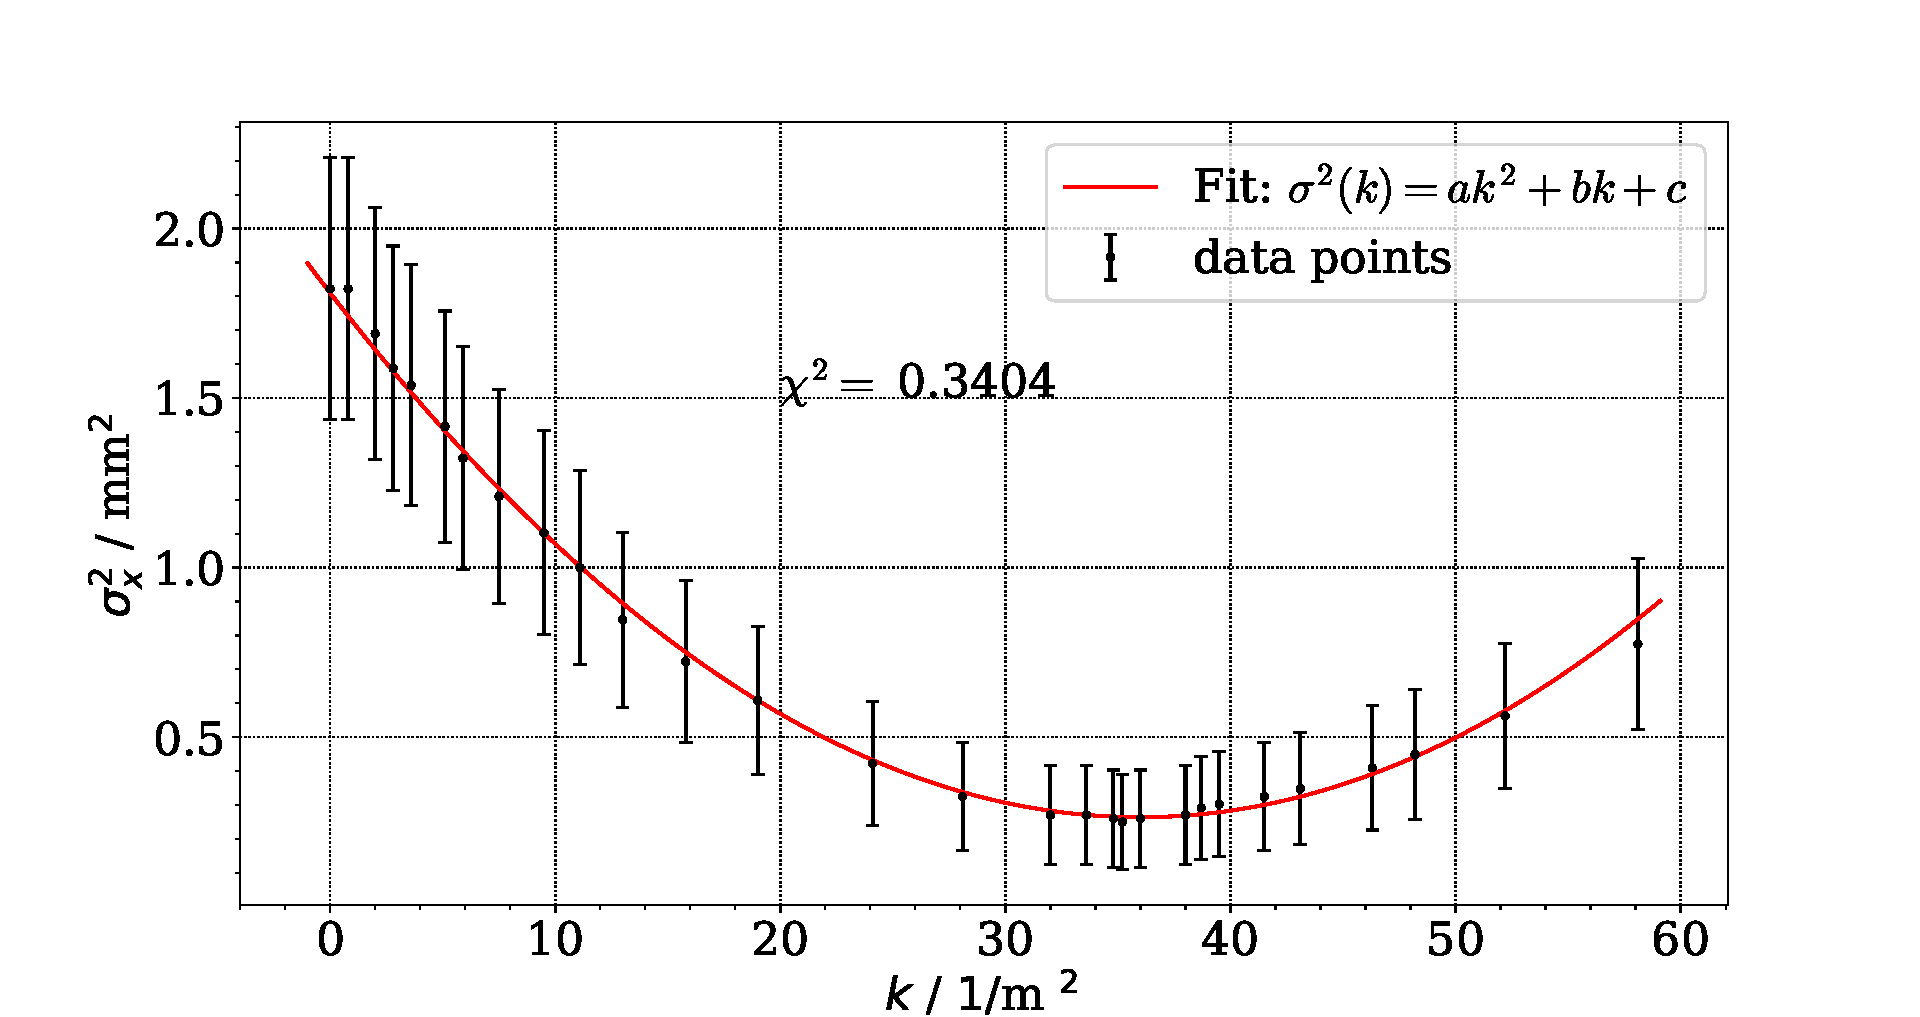
\includegraphics[width=\linewidth]{qscan_q1_x}
		\subcaption{horizontal width $\sigma_x^2(k)$}
	\end{subfigure}
	\begin{subfigure}{.49\linewidth}
		\includegraphics[width=\linewidth]{qscan_q1_z}
		\subcaption{vertical width $\sigma_z^2(k)$}
	\end{subfigure}
	\caption{Quadropole scan for quadropole Q1 and screen S1}
	\label{fig:qscan1}
\end{figure}
\begin{table}[htbp]
	\centering
	\begin{tabular}{c||cc}
		parameter& $x$& $z$\\
		\hline
		\hline

		$(\epsilon\alpha_0)$ /$\si{\milli\m^2\m^{-1}}$ &$0.202\pm0.014$ & $0.773\pm0.017$\\
		$(\epsilon\beta_0)$ /$\si{\milli\m^2}$ &$1.149\pm0.024$ & $1.359\pm0.025$\\
		$(\epsilon\gamma_0)$ /$\si{\milli\m^2\m^{-2}}$ &$1.579\pm0.03$ &$1.437\pm0.023$\\
		\hline
		\hline

		a / $\si{\milli\m^2\m^4}$ &$(1.194\pm0.020)\cdot10^{-3}$ &$(0.974\pm0.019)\cdot10^{-3}$ \\
		b / $\si{\milli\m^2\m^2}$&$(-85.94\pm1.12)\cdot10^{-3}$ &$(55.30\pm1.02)\cdot10^{-3}$\\
		c / $\si{\milli\m^2}$ &$1.81\pm0.016$ &$1.03\pm0.014$\\
	
		
	\end{tabular}
\caption{Fit results}
\label{tab:fitres1}
\end{table}
Our results of the twiss parameters are consistent with the solution obtained by solving the linear equation system with the benefit of a direct error on the parameters. We also see that there are no significant deviations from the quadratic formula in our data which is a nice result. Armed with $\epsilon\alpha,\epsilon\beta,\epsilon\gamma$ we can now determine the emittance.
\paragraph{Emittance via determinant}

Using equation \eqref{eq:det} one finds 

\begin{align*}
	\epsilon_x=\SI{1.332\pm0.019}{\milli\m\milli\radian} && \epsilon_z=\SI{1.164\pm0.024}{\milli\m\milli\radian}
\end{align*} 
\paragraph{Emmitance via beam waist}

The extremum of a quadratic function is given by \begin{align*}
	2ax+b=0\Leftrightarrow x=\hat{x}=-\frac{b}{2a}, && f(\hat{x})=-\frac{b^2}{4a}+c
\end{align*} and with this follows \begin{align*}
k_{w,x}=\SI{35.99 \pm 0.22 }{\m^{-2}}  &&\sigma_{w,x}^2=\SI{0.264\pm0.051}{\milli\m^2} && \epsilon_{x}=\SI{1.526\pm0.147}{\milli\m\milli\radian}
\end{align*}
as well as 
\begin{align*}
	k_{w,z}=\SI{-28.38 \pm 0.76 }{\m^{-2}}  &&\sigma_{w,z}^2=\SI{0.245\pm0.036}{\milli\m^2} && \epsilon_{z}=\SI{1.440\pm0.106}{\milli\m\milli\radian}.
\end{align*}
This agrees within a $2\sigma$ interval with our results obtained with the determinant method.


\subsubsection{Measurement at Screen S2}
We took the same measurements as before on Screen S2 with the second quadrople Q2. We turned the first quadropole off. Our data can be found in the appendix in tables \ref{tab:qscan2x},\ref{tab:qscan2z}. They are visualized in figure \ref{fig:qscan2}. We again have to determine the transformation matrix at the point S2 which is given by

$$M=M_\text{drift}M_{C2}M_\text{drift}M_\text{QF}M_{\text{drift}}M_{C1}M_\text{drift}M_\text{QF=0}M_{\text{drift}}M_{C0}=\begin{pmatrix}
	1-0.031413|k| &1.3865 - 0.0302193|k|\\
	-0.074|k| &1 - 0.071188|k|
\end{pmatrix}.$$
As mentioned before we turned the current through quadropole Q1 off. This is indicated by $M_{\text{QF}=0}$ in the above equation although we actually just stack the drift spaces there.

The fit results of the same functions as before are in table \ref{tab:fitres2}. The errors depicted will be discussed in subsection \ref{subsec:err}. 

\begin{figure}[htbp]
	\centering
	\begin{subfigure}{.49\linewidth}
		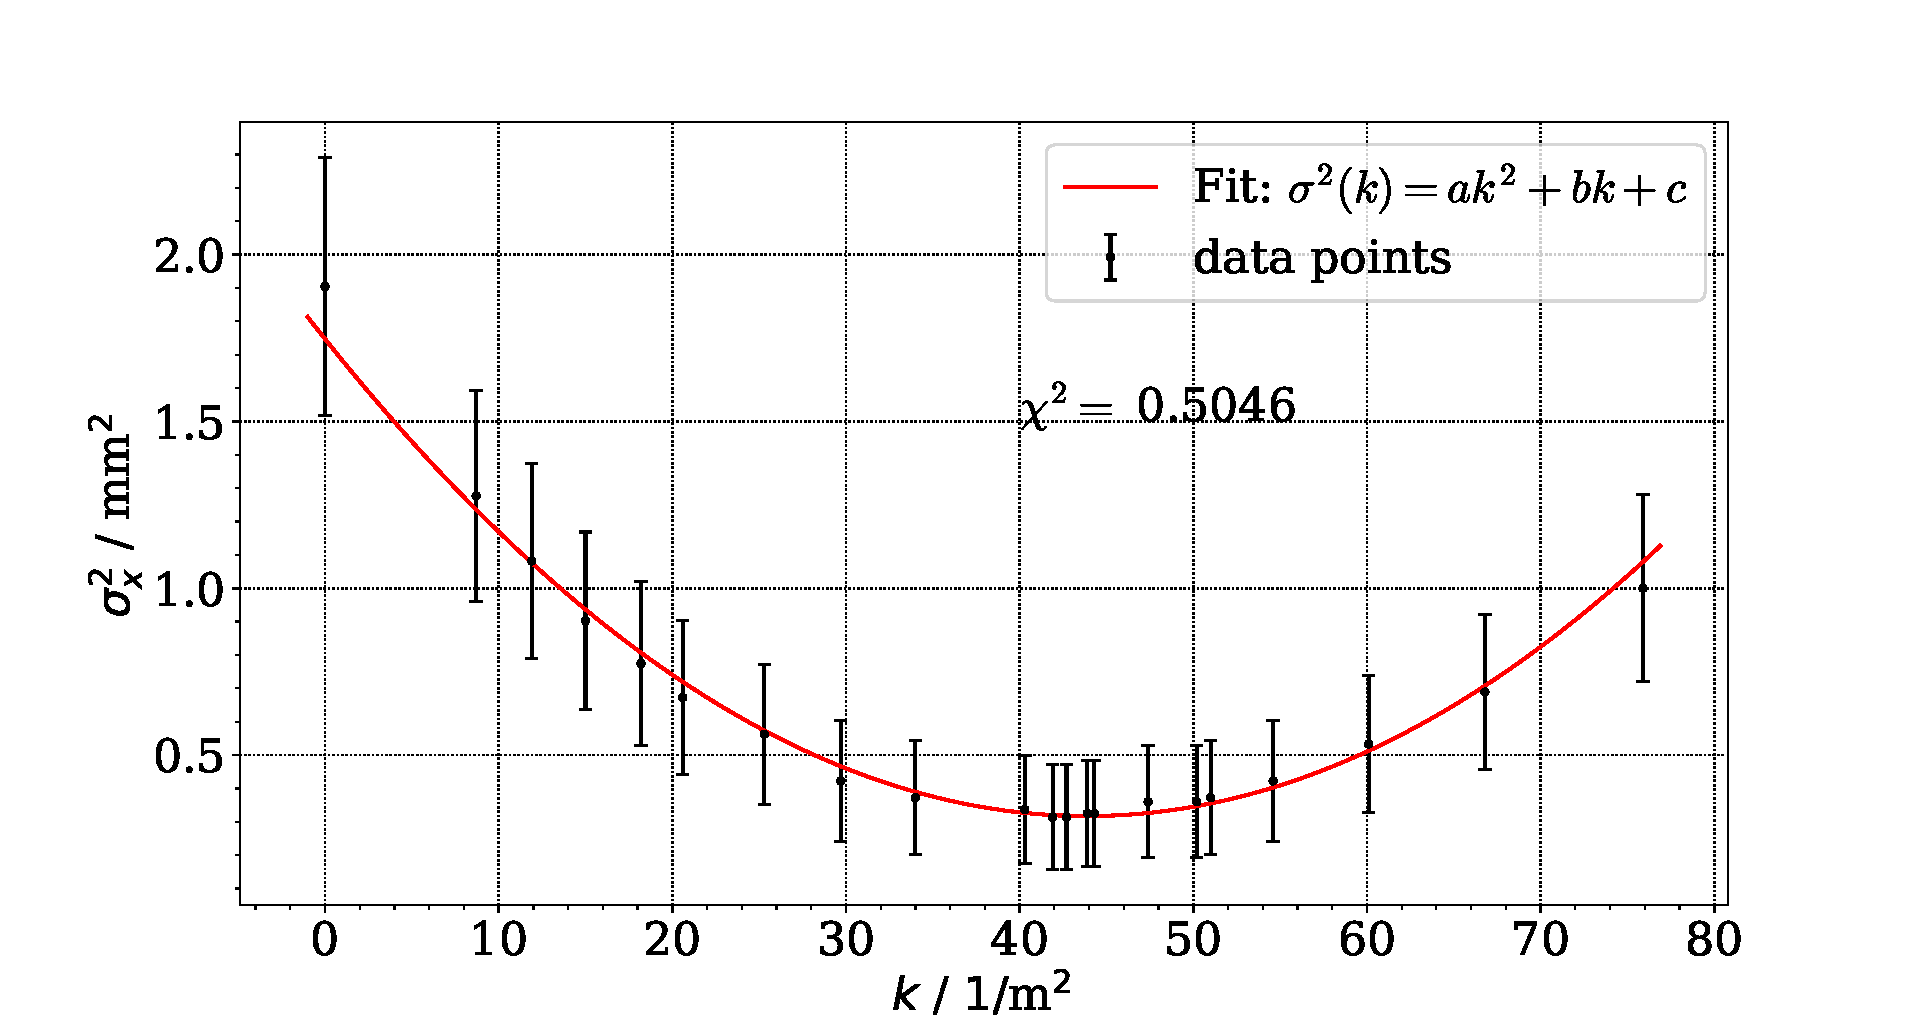
\includegraphics[width=\linewidth]{qscan_q2_x}
		\subcaption{horizontal width $\sigma_x^2(k)$}
	\end{subfigure}
	\begin{subfigure}{.49\linewidth}
		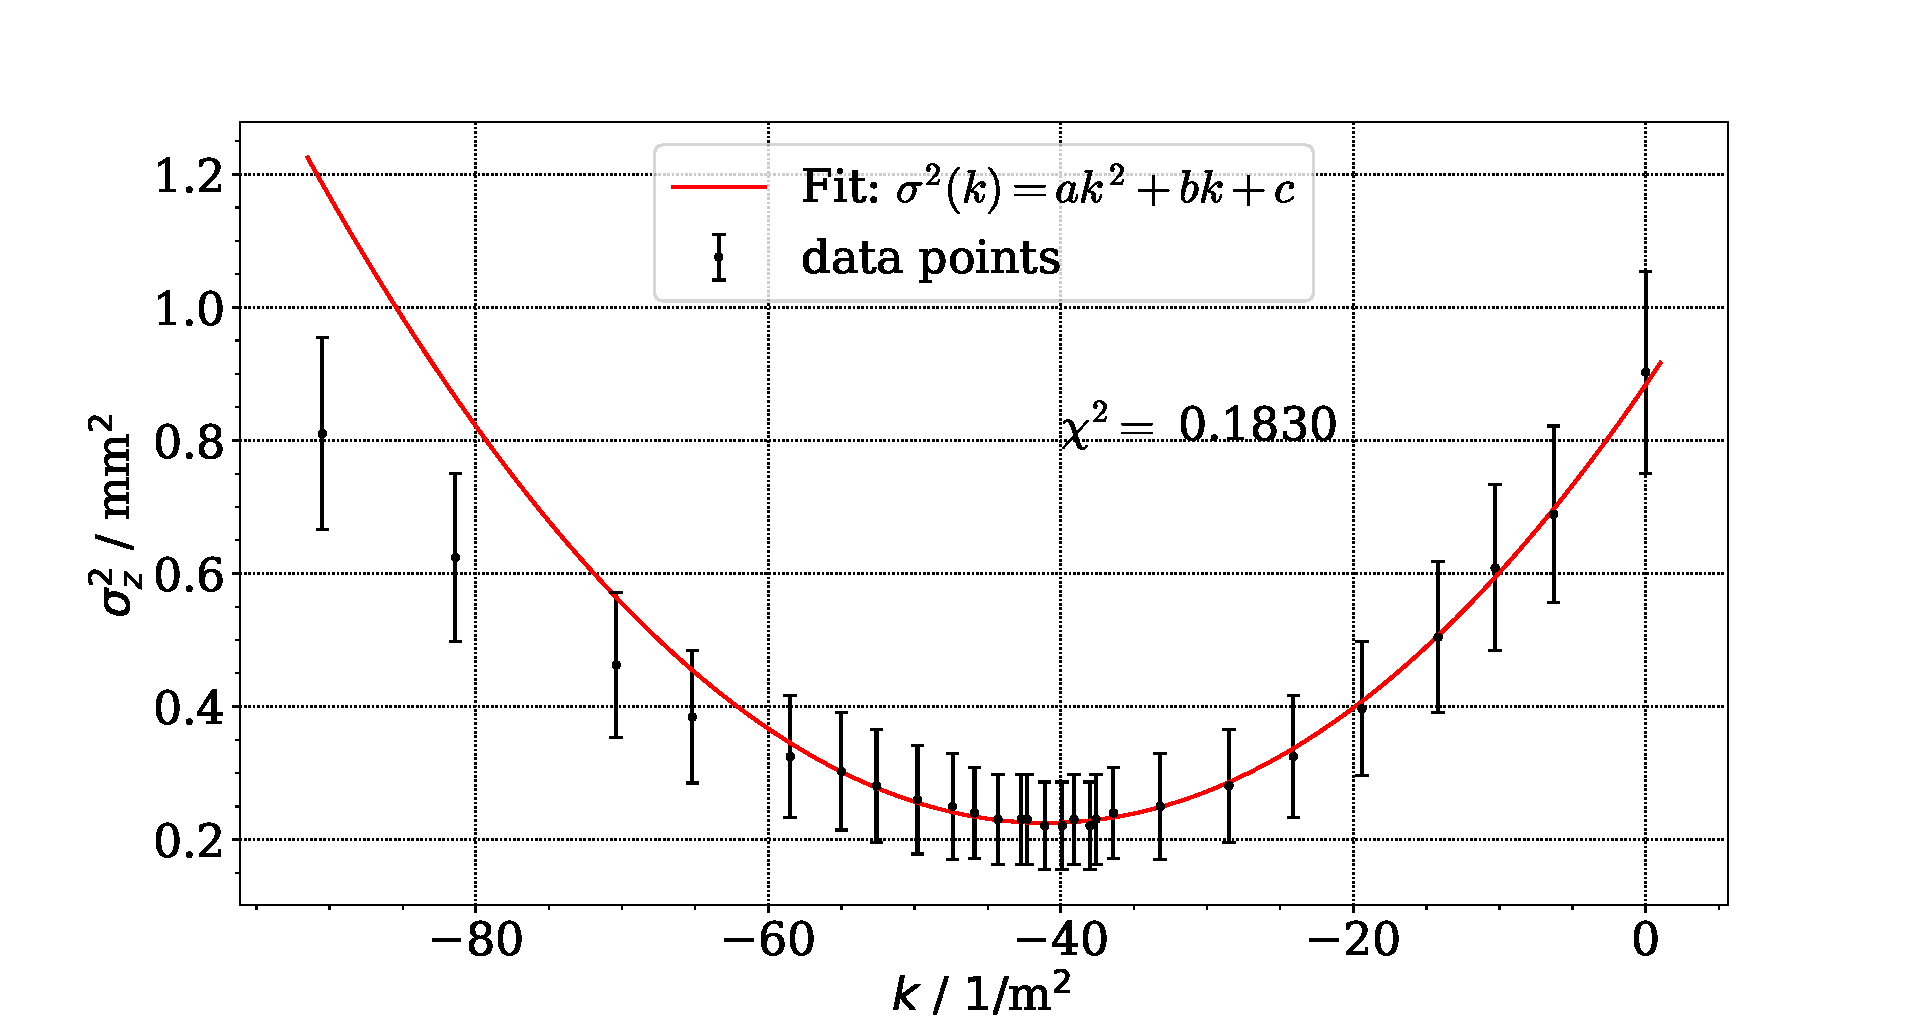
\includegraphics[width=\linewidth]{qscan_q2_z}
		\subcaption{vertical width $\sigma_z^2(k)$}
	\end{subfigure}
	\caption{Quadropole scan for quadropole Q2 and screen S2}
	\label{fig:qscan2}
\end{figure}
\begin{table}[htbp]
	\centering
	\begin{tabular}{c||cc}
		parameter& $x$& $z$\\
		\hline
		\hline

		$(\epsilon\alpha_0)$ /$\si{\milli\m^2\m^{-1}}$ &$1.597\pm0.050$ & $1.108\pm0.011$\\
		$(\epsilon\beta_0)$ /$\si{\milli\m^2}$ &$1.643\pm0.043$ & $1.204\pm0.010$\\
		$(\epsilon\gamma_0)$ /$\si{\milli\m^2\m^{-2}}$ &$2.357\pm0.052$ &$1.431\pm0.013$\\
		
		
		\hline
		\hline

		a / $\si{\milli\m^2\m^4}$ &$(0.743\pm0.022)\cdot10^{-3}$ &$(0.392\pm0.008)\cdot10^{-3}$ \\
		b / $\si{\milli\m^2\m^2}$&$(-65.19\pm1.76)\cdot10^{-3}$ &$(32.14\pm0.53)\cdot10^{-3}$\\
		c / $\si{\milli\m^2}$ &$1.75\pm0.035$ &$0.883\pm0.008$\\
		
	\end{tabular}
	\caption{Fit results}
	\label{tab:fitres2}
\end{table}

Again the crosscheck with the polynomial fit coefficients yielded no surprises. But now we see that for high $|k|>>1$ the measured width in vertical direction deviates significantly from a quadratic curve. Because of this we did not include the last four points in our fit. An explanation could be that at high quadropole strengths the focusing becomes so strong that our various assumptions and approximations (thin-lens, linear beam dynamics) are not valid anymore. 

Since we use the same reference point for both fits we should get similar results for the Twiss parameters, which we mostly do not get, especially in $x$ direction. This means that the matrices used do not describe the trajectory well enough. When we turned off the current for the quadrupole Q1 the software actually showed a finite remaining strength of $k_{\text{QF}\neq0}=\SI{-0.8}{m^{-2}}$ which will be investigated with the subscript $_{\text{QF}\neq0}$ in the remaining part of the analysis. Another reason for the not adequate description may be the neglecting of the impact of corrector magnets which are just assumed as drift lengths but we have no means to investigate this quantitatively.

Because $k_{\text{QF}\neq0}<0$ it focuses in vertical direction and we have to take into account two separate matrices for the propagation from $s_0$ to the screen $S2$ if we want to investigate its impact thoroughly.
\begin{align*}
	M_{\text{QF}\neq0}^x&=\begin{pmatrix}
		1.05618 - 0.0323884|k| & 1.33292 - 0.0282493|k|\\
		0.0592 - 0.0762977|k| & 1.02152 - 0.0665472|k|
	\end{pmatrix} \\ M_{\text{QF}\neq0}^z&=\begin{pmatrix}
	0.943819 - 0.0304376|k| & 1.29208 - 0.0275402|k|\\
	-0.0592 - 0.0717023|k| &0.978481 - 0.0648768|k| 
\end{pmatrix}
\end{align*}  

With the necessary matrix elements it is now possible to fit equation \eqref{eq:qscan} again to the data. The results are in table \ref{tab:fitres3}. 

\begin{table}[htbp]
	\centering
	\begin{tabular}{c||cc}
		parameter& $x$& $z$\\
		\hline
		\hline
		
		$(\epsilon\alpha_0)$ /$\si{\milli\m^2\m^{-1}}$ &$1.489\pm0.048$ & $0.952\pm0.010$\\
		$(\epsilon\beta_0)$ /$\si{\milli\m^2}$ &$1.459\pm0.038$ & $1.102\pm0.008$\\
		$(\epsilon\gamma_0)$ /$\si{\milli\m^2\m^{-2}}$ &$2.426\pm0.055$ &$1.376\pm0.012$\\
		
		
	\end{tabular}
	\caption{Fit results}
	\label{tab:fitres3}
\end{table}

We see partially only mild improvement and partially even worsening which means that the deviance from our expected values must stem from another source as discussed above. We will use the results from table \ref{tab:fitres2} in the following since the influence of the remaining quadrupole strength is not really significant.
\paragraph{Concluding remark regarding the Twiss parameters}
Although due to some systematical/methodical error we can not exactly reproduce the Twiss parameters after the first corrector but we can reconstruct their order of magnitude correctly and their signs match. This means that roughly the beam properties are determined the same from two different measurement points.
\paragraph{Emittance via determinant}

Again we use equation \eqref{eq:det} to determine the emittance
\begin{align*}
	\epsilon_x=\SI{1.150\pm0.090}{\milli\m\milli\radian} && \epsilon_z=\SI{0.704\pm0.088}{\milli\m\milli\radian}
\end{align*} 
\paragraph{Emittance via beam waist}
Using the same strategy as before we find
\begin{align*}
	k_{w,x}=\SI{43.87 \pm 0.18 }{\m^{-2}}  &&\sigma_{w,x}^2=\SI{0.320\pm0.095}{\milli\m^2} && \epsilon_{x}=\SI{1.383\pm0.117}{\milli\m\milli\radian}
\end{align*}
as well as 
\begin{align*}
	k_{w,z}=\SI{-41.00 \pm 0.11 }{\m^{-2}}  &&\sigma_{w,z}^2=\SI{0.224\pm0.027}{\milli\m^2} && \epsilon_{z}=\SI{0.911\pm0.109}{\milli\m\milli\radian},
\end{align*}
again agreeing with the values obtained with the determinant method in approximately two standard deviations.
\subsubsection{Comparing the results at both Screens}
Before stepping further and determining the emittance via the multiscreen method let us recapitulate our results so far. They are depicted in table \ref{tab:res1}. We see that the error obtained with the determinant method are smaller by a factor of ten. This leads to agreement between the results obtained at S1 and S2 within $2\sigma$ while the beam waist method provides agreement within a $1\sigma$ interval. This only holds for the emittance in horizontal direction. In vertical direction the deviations are significantly larger. Here only the results obtained at one respective screen agree within $2\sigma$. Generally the emittance is estimated smaller further away from the point where we want to measure it. This makes sense since the beam has propagated longer and may have suffered losses which are not describable by ion optics which we had to assume a priori.

\begin{table}[htbp]
	\centering
	\begin{tabular}{c||cc|cc||c}
		
		method&\multicolumn{2}{c|}{determinant} & \multicolumn{2}{c||}{beam waist}& mean\\
		measured at&S1 & S2& S1 & S2&\\
		\hline
		$\epsilon_{x}$ / \si{\milli\m\milli\radian} &$\SI{1.332\pm0.019}{}$&$\SI{1.150\pm0.090}{}$&$\SI{1.526\pm0.147}{}$&$\SI{1.383\pm0.117}{}$&$1.348\pm0.052$\\
		\hline
		\hline
		$\epsilon_{z}$ / \si{\milli\m\milli\radian} &$\SI{1.164\pm0.024}{}$&$\SI{0.704\pm0.088}{}$&$\SI{1.440\pm0.106}{}$&$\SI{0.911\pm0.109}{}$&$1.050\pm0.044$\\

	\end{tabular}
	
	\caption{Results of emittance at Screen S1 and S2}
	\label{tab:res1}
\end{table}




\subsection{Multiscreen-method}
\label{subsec:msc}
Instead of measuring the beam width $\sigma_\xi(k)$ we can measure $\sigma_\xi$ at all available screens with constant quadropole strength and obtain a set of linear equations using equation \eqref{eq:beta} which is given in equation \eqref{eq:multiscreen} \cite{script}
\begin{equation}
	\underbrace{
	\begin{pmatrix}
		\sigma^2(s_0)\\
		\sigma^2(s_1)\\
		\sigma^2(s_2)\\
		\sigma^2(s_3)\\
		\sigma^2(s_4)\\
	\end{pmatrix}}_{\vec{\sigma}}
	=\underbrace{\begin{pmatrix}
		m_{11}^2(s_0) & -2m_{11}(s_0)\cdot m_{12}(s_0) & m_{12}^2(s_0)\\
		m_{11}^2(s_1) & -2m_{11}(s_1)\cdot m_{12}(s_1) & m_{12}^2(s_1)\\
		m_{11}^2(s_2) & -2m_{11}(s_2)\cdot m_{12}(s_2) & m_{12}^2(s_2)\\
		m_{11}^2(s_3) & -2m_{11}(s_3)\cdot m_{12}(s_3) & m_{12}^2(s_3)\\
		m_{11}^2(s_4) & -2m_{11}(s_4)\cdot m_{12}(s_4) & m_{12}^2(s_4)\\
	\end{pmatrix}}_{\mathcal{M}}
	\cdot
	\underbrace{
	\begin{pmatrix}
		\epsilon\alpha_0\\
		\epsilon\beta_0\\
		\epsilon\gamma_0\\
	\end{pmatrix}}_{\vec{\chi}},
	\label{eq:multiscreen}
\end{equation}
where $m_{ij}(s_n)$ are the transition matrix elements at screens $S0$ -- $S4$ and $\sigma^2(s_n)$ the squared widths at the respective screens. One can solve this equation system by solving the equation $$\mathcal{M}^T\cdot\vec{\sigma}=(\mathcal{M}^T\cdot\mathcal{M})\cdot\vec{\chi}.$$ 
We measured the horizontal and vertical widths at all screens with all quadrupoles turned off, see table \ref{tab:datascreen}. 
\begin{table}[htbp]
	\centering
	\begin{tabular}{c|c|c}
		Screen &   $\sigma_x$ / mm   & $\sigma_z$ / mm \\
		\hline
		\hline
		0      &   1.04      & 0.88    \\
		1      &   1.36      & 1.03    \\
		2      &   1.36      & 0.89    \\
		3      &   1.73      & 1.05    \\
		4      &   2.51      & 1.55   
	\end{tabular}
\caption{Widths measured at all screens}
\label{tab:datascreen}
\end{table}


This means that at every screen the transition matrices are given by a drift matrix with the right propagation length \textbf{from the same starting point $\mathbf{ s_0}$ as in the previous subsection}. We will not explicitly list them here. We use again \emph{Wolfram Mathematica} to solve equations we do not want to solve by hand and obtain the results 
\begin{align*}
	\vec{\chi_x}=\begin{pmatrix}
		(\epsilon\beta_0)\\
		(\epsilon\alpha_0)\\
		(\epsilon\gamma_0)\\
	\end{pmatrix}=\begin{pmatrix}
	\SI{1.746}{\milli\m^2}\\
	\SI{0.844}{\milli m^2m^{-1}}\\
	\SI{1.240}{\milli m^2m^{-2}}
\end{pmatrix} && \epsilon_{x}=\SI{1.205\pm0.034}{\milli\m\milli\radian}\\
\vec{\chi_z}=\begin{pmatrix}
	(\epsilon\beta_0)\\
	(\epsilon\alpha_0)\\
	(\epsilon\gamma_0)\\
\end{pmatrix}=\begin{pmatrix}
	\SI{1.158}{\milli\m^2}\\
	\SI{0.484}{\milli m^2m^{-1}}\\
	\SI{0.520}{\milli m^2m^{-2}}
\end{pmatrix} && \epsilon_{z}=\SI{0.607\pm0.091}{\milli\m\milli\radian}
\end{align*}
If we solve the equations with the widths plus and minus their error, see subsection \ref{subsec:err}, we can estimate an error on our result, which is only systematical and not statistical. We can not propagate errors through an equation solving algorithm. The results obtained via the multiscreen method agree within a few standard deviations with our previous results. Nevertheless the emittance is estimated smaller than before. Also the Twiss parameters are only representing very roughly the same beam properties at our starting point $s_0$. As all quadrupoles were turned off we measured, as before, a finite remaining field strength of $k_{\text{QF}\neq0}=\SI{-0.8}{\m^{-2}}$. If we consider this we have to alter our transition matrices accordingly and obtain 
\begin{align*}
	\vec{\chi_x}=\begin{pmatrix}
		(\epsilon\beta_0)\\
		(\epsilon\alpha_0)\\
		(\epsilon\gamma_0)\\
	\end{pmatrix}=\begin{pmatrix}
		\SI{1.725}{\milli\m^2}\\
		\SI{0.873}{\milli m^2m^{-1}}\\
		\SI{1.341}{\milli m^2m^{-2}}
	\end{pmatrix} && \epsilon_{x}=\SI{1.246\pm0.064}{\milli\m\milli\radian}\\
	\vec{\chi_z}=\begin{pmatrix}
		(\epsilon\beta_0)\\
		(\epsilon\alpha_0)\\
		(\epsilon\gamma_0)\\
	\end{pmatrix}=\begin{pmatrix}
		\SI{1.212}{\milli\m^2}\\
		\SI{0.595}{\milli m^2m^{-1}}\\
		\SI{0.755}{\milli m^2m^{-2}}
	\end{pmatrix} && \epsilon_{z}=\SI{0.750\pm0.113}{\milli\m\milli\radian}.
\end{align*}
As those results agree better with our previous results we will use them in further discussions. In principle all remarks about their properties remain the same as before with the difference that we agree within a smaller error margin with the previous results.

\subsection{Discussion of measured beam properties}
We calculated the beam emittance and twiss parameters in various ways in the previous sections. We shall now visualize our findings by plotting the horizontal and vertical phase space ellipse. The phase space equation reads \cite{wille} 
\begin{equation}
	\epsilon_\xi(s)\left[\gamma_\xi(s)\xi^2(s)+2\alpha_\xi(s)\xi(s)\cdot\xi'(s)+\beta_\xi(s)\xi'^2(s)\right]=\epsilon_\xi^2(s),	
\end{equation}
which we can evaluate at $s=s_0$. Figure \ref{fig:phasespace} shows the resulting ellipses of our results from the quadrupole scan method (subsection \ref{subsec:qscan}) and of the multiscreen method (subsection \ref{subsec:msc}). All are normed to the same emittance which was calculated as the mean of the result from the quadrupole-scan method and the multiscreen method. In both cases the phase space ellipse is estimated only very roughly the same by the different methods used to determine the beam parameters. Especially the quadrupole scan method at screen S2 seems to have suffered some significant systematical error along its propagation which we could not account for in the process of our analysis. A nice result however is that the multiscreen method seems to fit right between the other two estimates indicating that, at least in general, we measured the "same" beam properties; there are no vast surprises regarding the ellipse orientation and overall form. 

\begin{figure}[H]
	\centering
	\begin{subfigure}{.49\linewidth}
		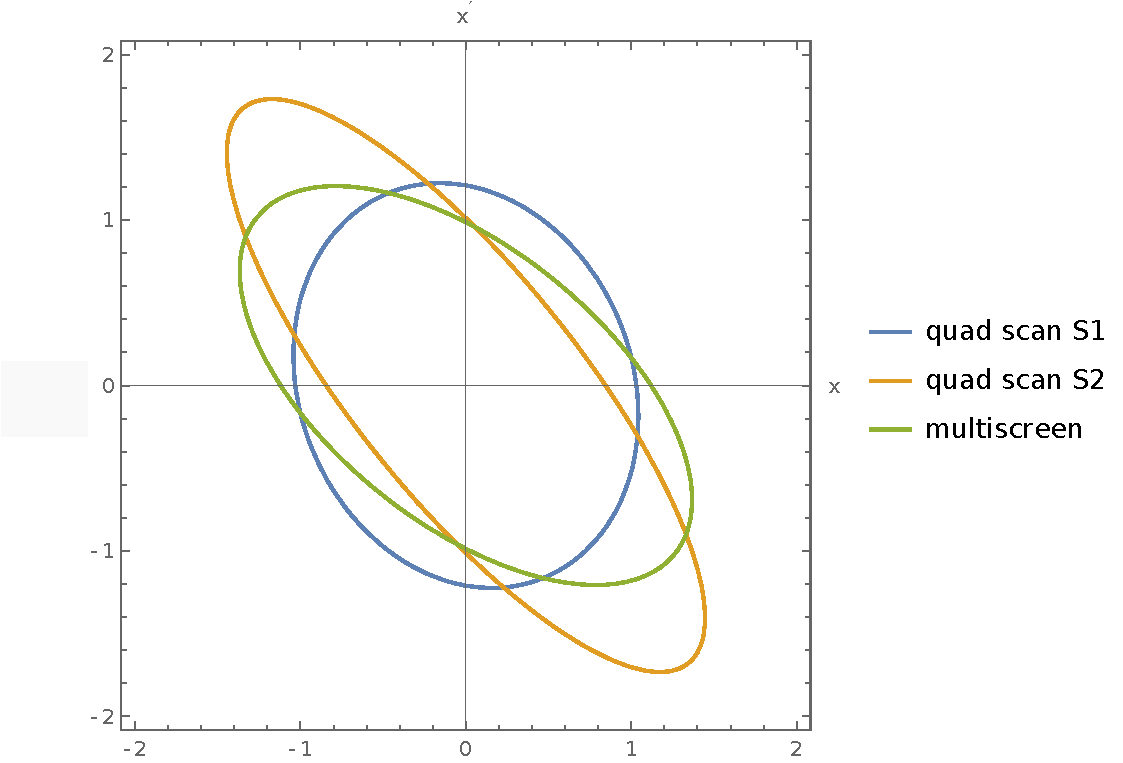
\includegraphics[width=\linewidth]{figs/horizontal_phasespace.pdf}
		\subcaption{horizontal}
	\end{subfigure}
\begin{subfigure}{.49\linewidth}
	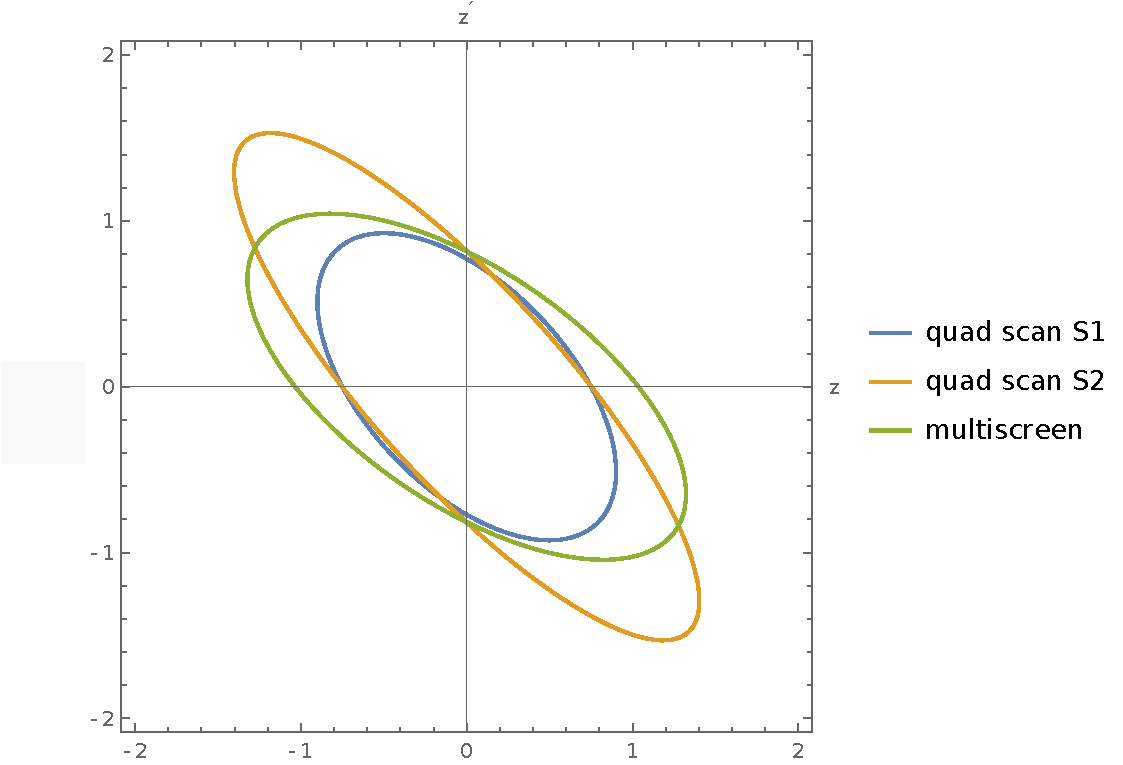
\includegraphics[width=\linewidth]{figs/vertical_phasespace.pdf}
	\subcaption{vertical}
\end{subfigure}
\caption{Phase space ellipses visualizing our results of the beam properties}
\label{fig:phasespace}
\end{figure} 
We can thus make the following general remarks about the beam at our reference point $s_0$

\begin{itemize}
	\item the beam leaves the corrector neither at a beam waist nor at a focusing point, otherwise the ellipses would be upright \cite{wille} 
	\item the beam covers an area of approximately $2\times2$ mm
	\item the beam has approximately the same properties in horizontal and vertical direction
\end{itemize}


\subsection{Discussion of systematic errors}
\label{subsec:err}
In previous sections we applied systematic errors. We derived them by scanning the last screen S4 by varying the kick angle $\alpha$ of the last corrector magnet C4. We therefore measured the beam position and the beam widths and took the standard deviation of this distribution. This systematic error shall be a simple approach and gives a first estimation. Table \ref{tab:sys_error} lists all measurements.

\begin{table}[H]
	\centering
	\begin{tabular}{|c|c|c|c|}
		\hline
		$x$ / mm &	$\sigma_x$ / mm	&$y$ / mm&	$\sigma_y$ / mm\\
		\hline
		0.66&	1.3	&-4.16&	1.01 \\
		-8.86&	1.19&	-4.13	&0.85 \\
		12.11&	1.18&	-4.06	&0.85 \\
		1.66&	1.49&	4.62	&0.91 \\
		0.35&	0.87&	-10.73&	0.67 \\
		8.10&	0.89&	-10.47&	0.67 \\
		-4.55&	0.87&	-10.57&	0.65 \\
		\hline
	\end{tabular}
	\caption{Measurement of beam-position dependence}\label{tab:sys_error}
\end{table}
Calculating the mean and the standard derivation for the first 4 values one finds
\begin{align*}
	\hat\sigma_x=1.29&& \text{std}(\sigma_x)=0.14&& \text{ and } &&\hat\sigma_z=0.91&&\text{std}(\sigma_z)=0.07.
\end{align*}
We dropped the last three measurements at high values of $y$ because the the beam distortion was rather high in comparison. Also the beam wasn't focused to the edges of the screen as seen in figure \ref{fig:Screenshots}. We also conclude from the various fits we did before that the error was estimated \emph{very} (too) generously which we can conclude from the very small values of $\chi^2$ obtained from the quadratic fits. It would have been better to select a smaller region around the center of the beam and derive a standard deviation from this and not take the extreme outer regions. Nevertheless we took this error as we lacked any other estimate apart from statistical fluctuations around the fitted value which do not represent any real error. As mentioned before of course all our set values of kick angles do influence our results and any error there will be a systematic error on the results which can not be accounted for. In principle a thorough investigation would demand analyzing all possible parameter sets inside of estimated errors and doing the whole analysis provided so far each time, which is beyond the scope and available time of this lab course. But one can say we took this into account by assigning such a generous error on the measured widths. We regret not measuring the systematic error coming with various beam intensities on the different screens, this would have been an interesting addition to our estimate of a systematical error. Also a more thorough investigation of a systematic error like we used should consider in principle each screen individually which again time did not permit.
\newpage
\section{Conclusion}
\label{sec:conc}
In this lab course we investigated the  Lab course Accelerator or short LAB. After getting used to the control software we started with a beam calibration by eye. 

In our first measurement we verified the linear relation between the kick angle $\alpha$ and the beam position in the first two corrector magnets. Additionally we verified the expected linear relation between the current and the kick angle. 

We then aligned the particle beam by measuring the beam offset after each quadrupole with varying quadrupole strengths $k$ and the applied kick angle $\alpha$. With a linear fit for the beam offset $\Delta x(\alpha_x), \Delta z(\alpha_z)$ we found the ideal kick angles, so that the quadrupole should only have an influence on the beam focus and not on the position. Now we were ready to measure the beam emittance $\epsilon$ by two methods.

The first method was the quadrupole scan. Therefore we measured the beam width $\sigma_{x,z}$ in dependence of the quadrupole strength $k$. We then plotted the square of $\sigma_{x,z}$ against $k$ and fitted a polynomial of second order. By applying some matrix optics we derived the emittance via the determinant of the beta matrix as well via the beam waist. Our results for the screens S1 and S2 are
\begin{table}[H]
	\centering
	\begin{tabular}{c||cc|cc||c}
		
		method&\multicolumn{2}{c|}{determinant} & \multicolumn{2}{c||}{beam waist}& mean\\
		measured at&S1 & S2& S1 & S2&\\
		\hline
		$\epsilon_{x}$ / \si{\milli\m\milli\radian} &$\SI{1.332\pm0.019}{}$&$\SI{1.150\pm0.090}{}$&$\SI{1.526\pm0.147}{}$&$\SI{1.383\pm0.117}{}$&$1.348\pm0.052$\\
		\hline
		\hline
		$\epsilon_{z}$ / \si{\milli\m\milli\radian} &$\SI{1.164\pm0.024}{}$&$\SI{0.704\pm0.088}{}$&$\SI{1.440\pm0.106}{}$&$\SI{0.911\pm0.109}{}$&$1.050\pm0.044$\\
		
	\end{tabular}
	
	\caption*{}
\end{table}

For the multiscreen method we measured the beam width $\sigma_\xi(k)$ at all available screens with constant quadropole strength $k=\text{const.}$ and obtained a set of linear equations. One can solve this system of linear equations and derive the emittance $\epsilon$
\begin{align*}
\epsilon_{x}=\SI{1.246\pm0.064}{\milli\m\milli\radian}  && \epsilon_{z}=\SI{0.750\pm0.113}{\milli\m\milli\radian}.
\end{align*}

These results now do coincide with the results above within $1\sigma$ for the horizontal emittance and within $2\sigma$ for the vertical emittance, which is nice. 

Along the way of computing the emittance we gained insight in the measured beam properties by visualizing the beam parameters in phase space and obtained (rather) satisfactory findings which however beg further investigations that overshoot the ambitions of this lab course.
\newpage
\appendix\section{Appendix}\label{sec:Appendix}
\counterwithin{figure}{section}
\counterwithin{table}{section}
\begin{table}[htbp]
	\centering
	\begin{tabular}{|l|l|l|}
		\hline
		name  & type       & length / m \\
		\hline
		C0    & corrector  & 0.0785     \\
		& drift      & 0.185      \\
		S0-S4 & screen     & 0.04       \\
		& drift      & 0.06       \\
		Q1-Q4 & quadrupole & 0.074      \\
		& drift      & 0.03       \\
		C1-C4 & corrector  & 0.0785     \\
		& drift      & 0.316     \\
		\hline
	\end{tabular}
\caption{Dimensions of the optical elements \cite{script}}\label{tab:LAB_dimensions}
\end{table}
\subsection{Additional verifications}\label{sec:additional_verficitation}
To verify of what should be clear, we plotted the kick angle $\alpha$ against the current and found the expected linear relation. Figure \ref{fig:qual_plot} only shows a qualitative result without errorbars. With this result follows the same qualitative course as in figure \ref{fig:kick_verify} for the current against the position $x$,$y$. This is depicted in figure \ref{fig:current_verify}.
\begin{figure}[H]
	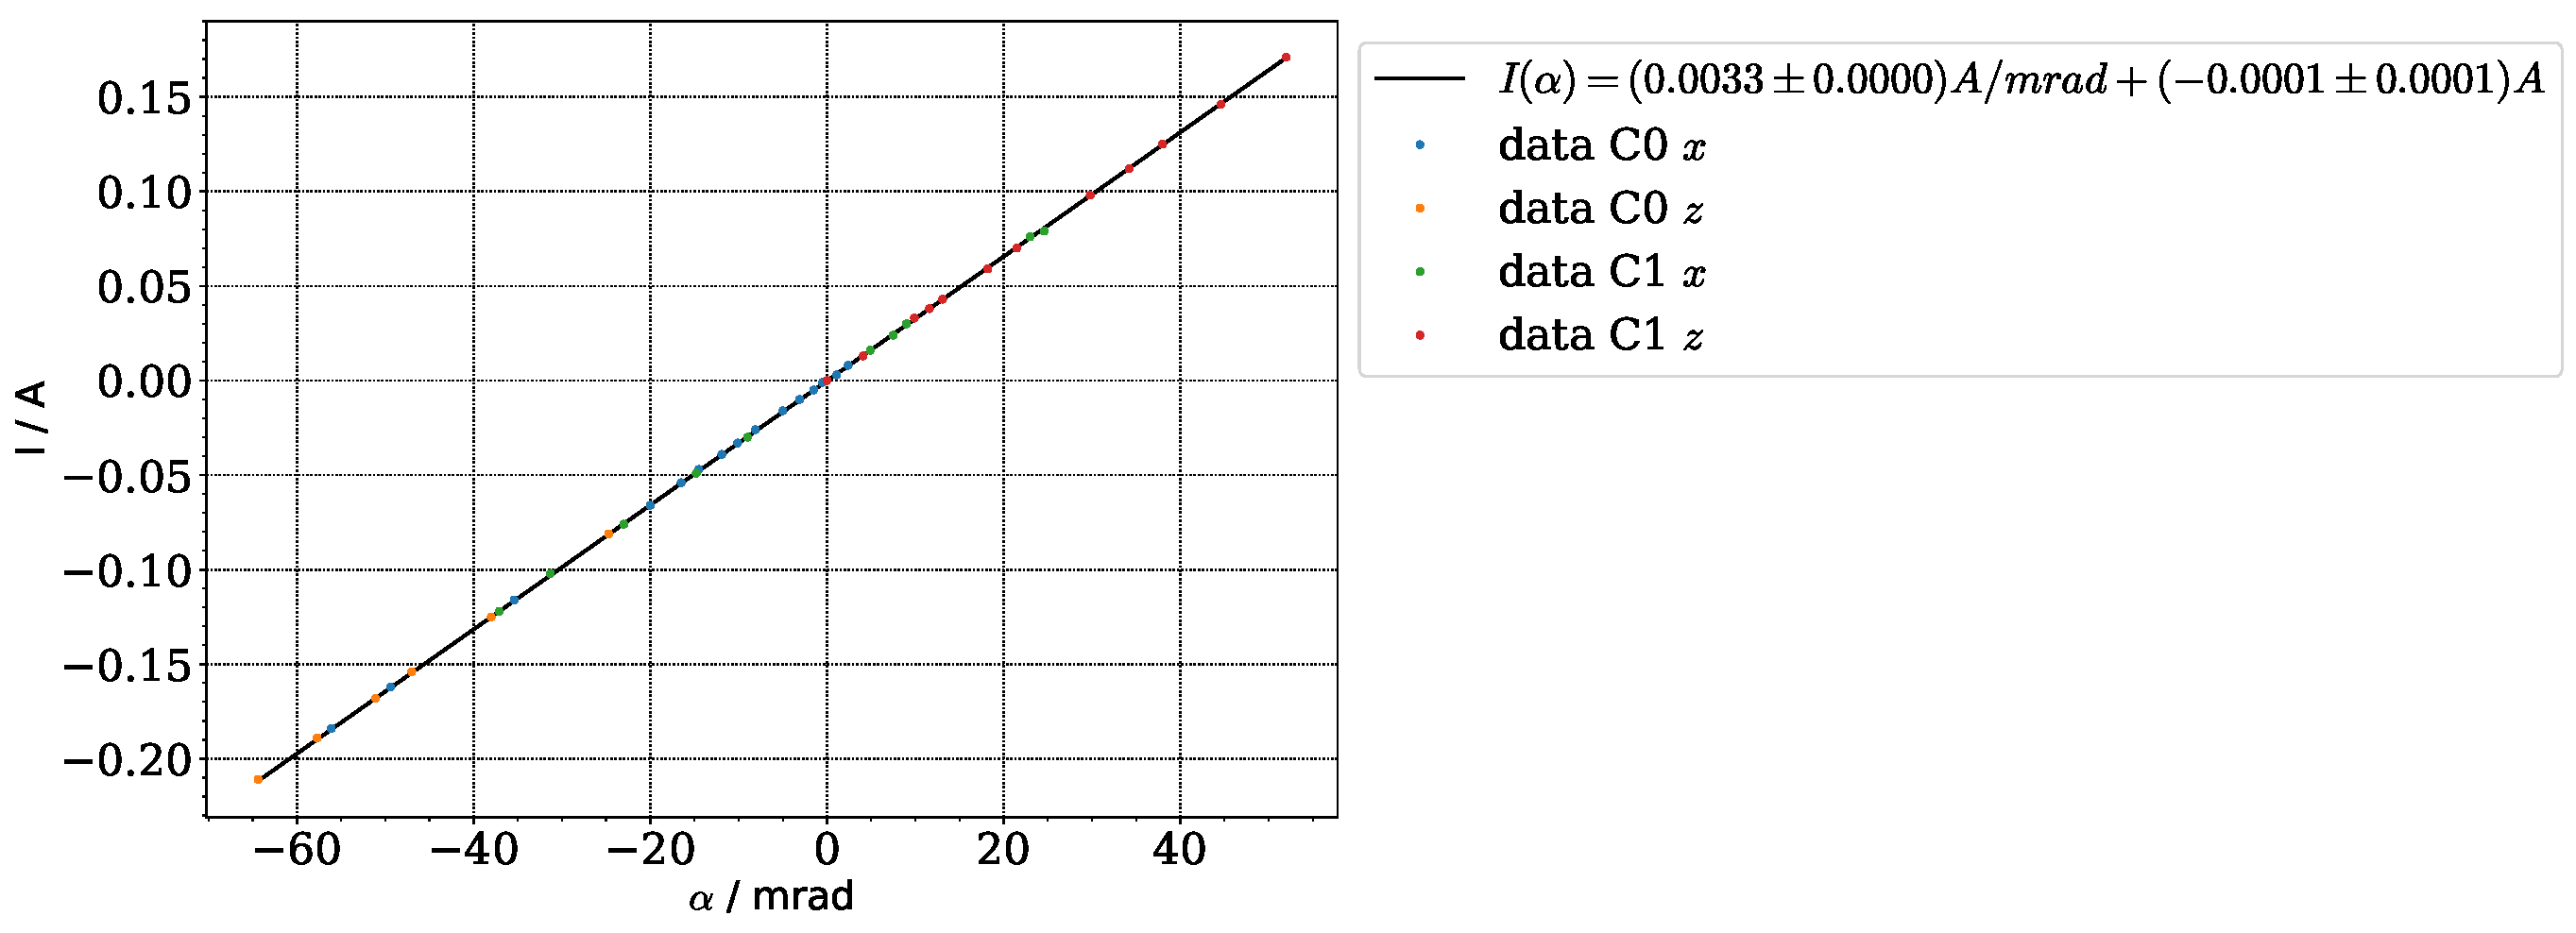
\includegraphics[width=\linewidth]{figs/calibration/current_vs_kick.pdf}
	\caption{Qualitative fit of the kick angle $\alpha$ against the applied current}\label{fig:qual_plot}
\end{figure}
\begin{figure}[H]
	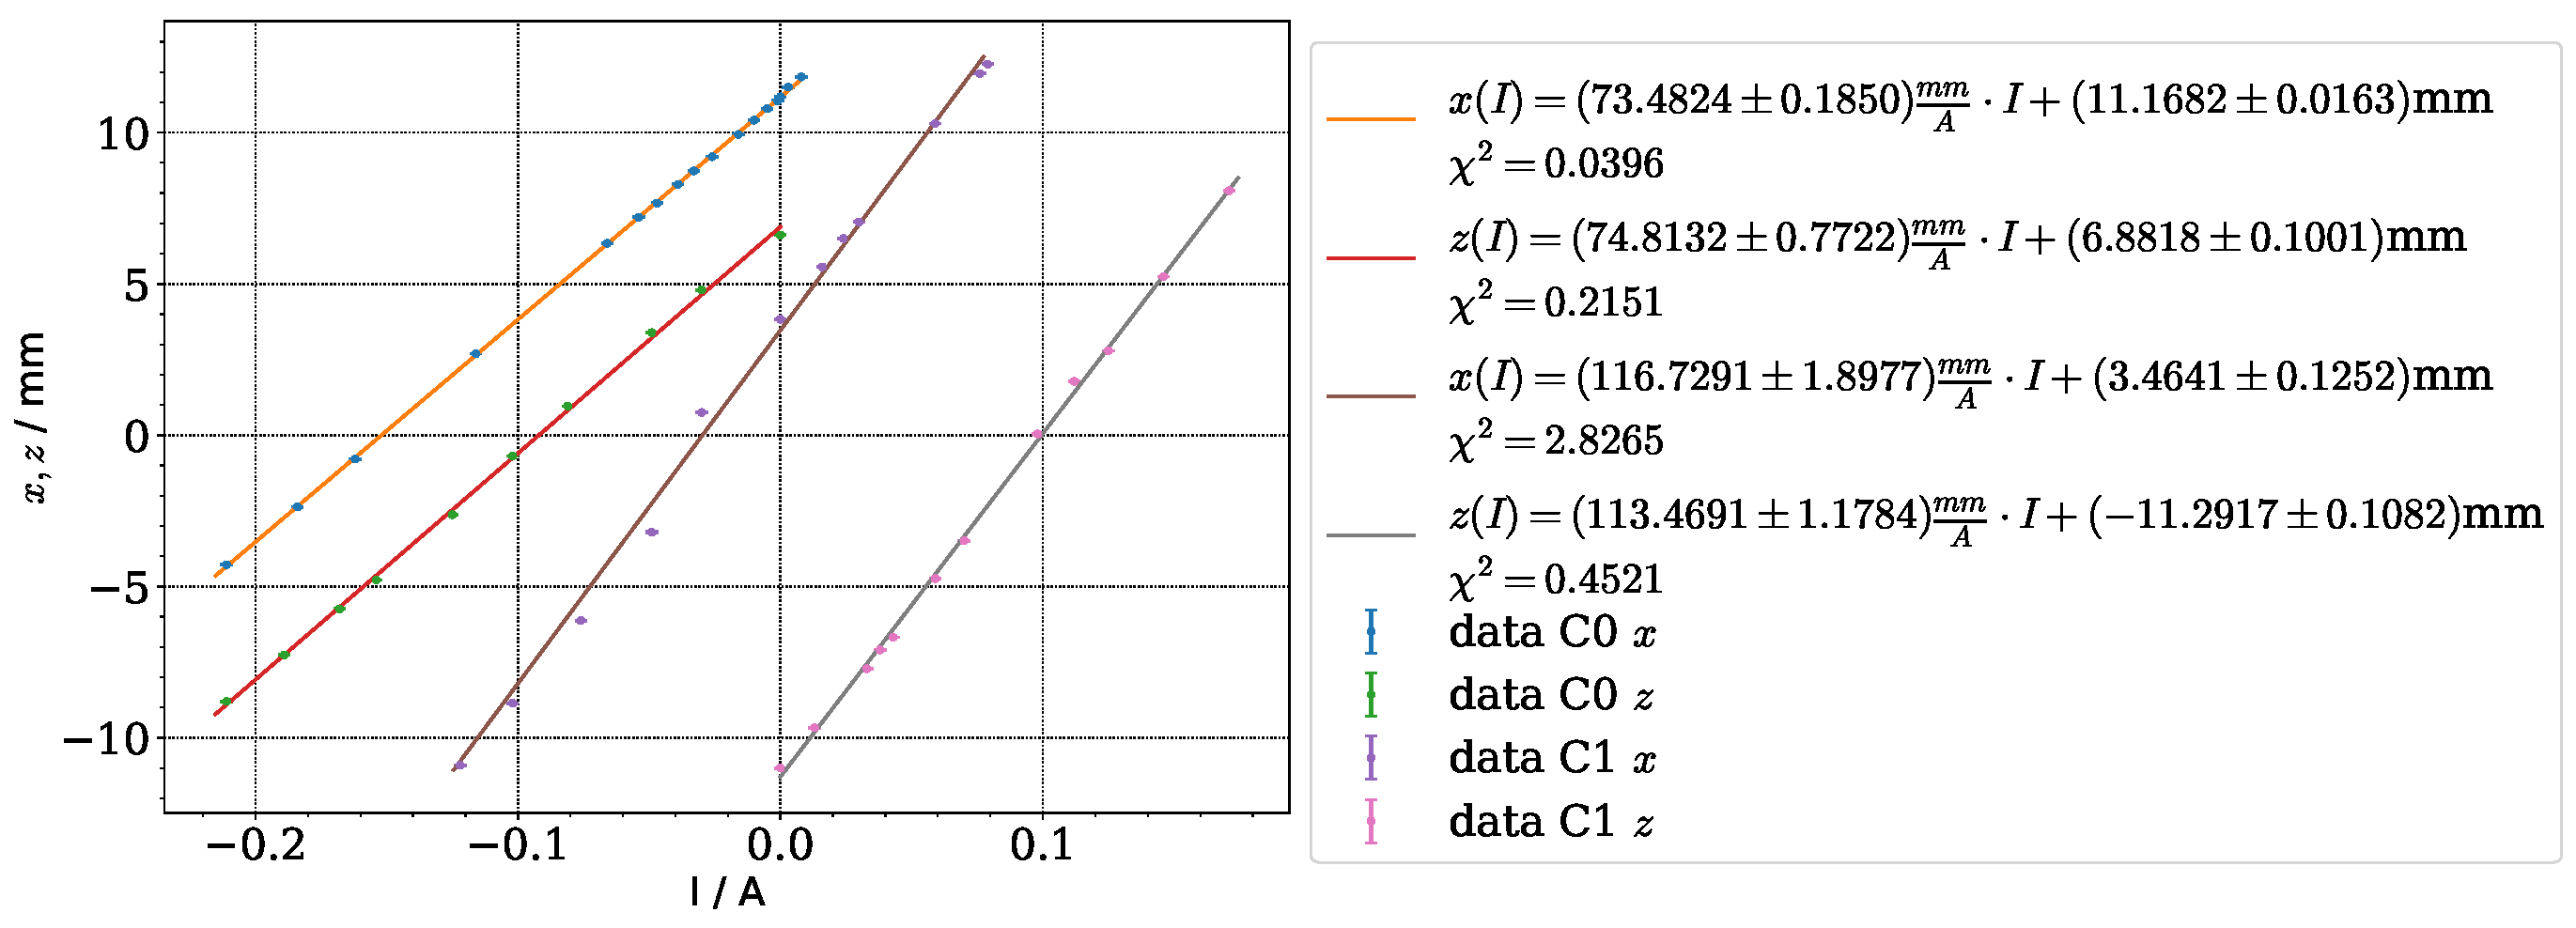
\includegraphics[width=\linewidth]{figs/calibration/current_verification.pdf}
	\caption{Additional plot of the beam position $x$,$y$ dependent on the current $I$}\label{fig:current_verify}
\end{figure}
\begin{figure}
	\vspace{-.5cm}
	\begin{subfigure}{.49\linewidth}
		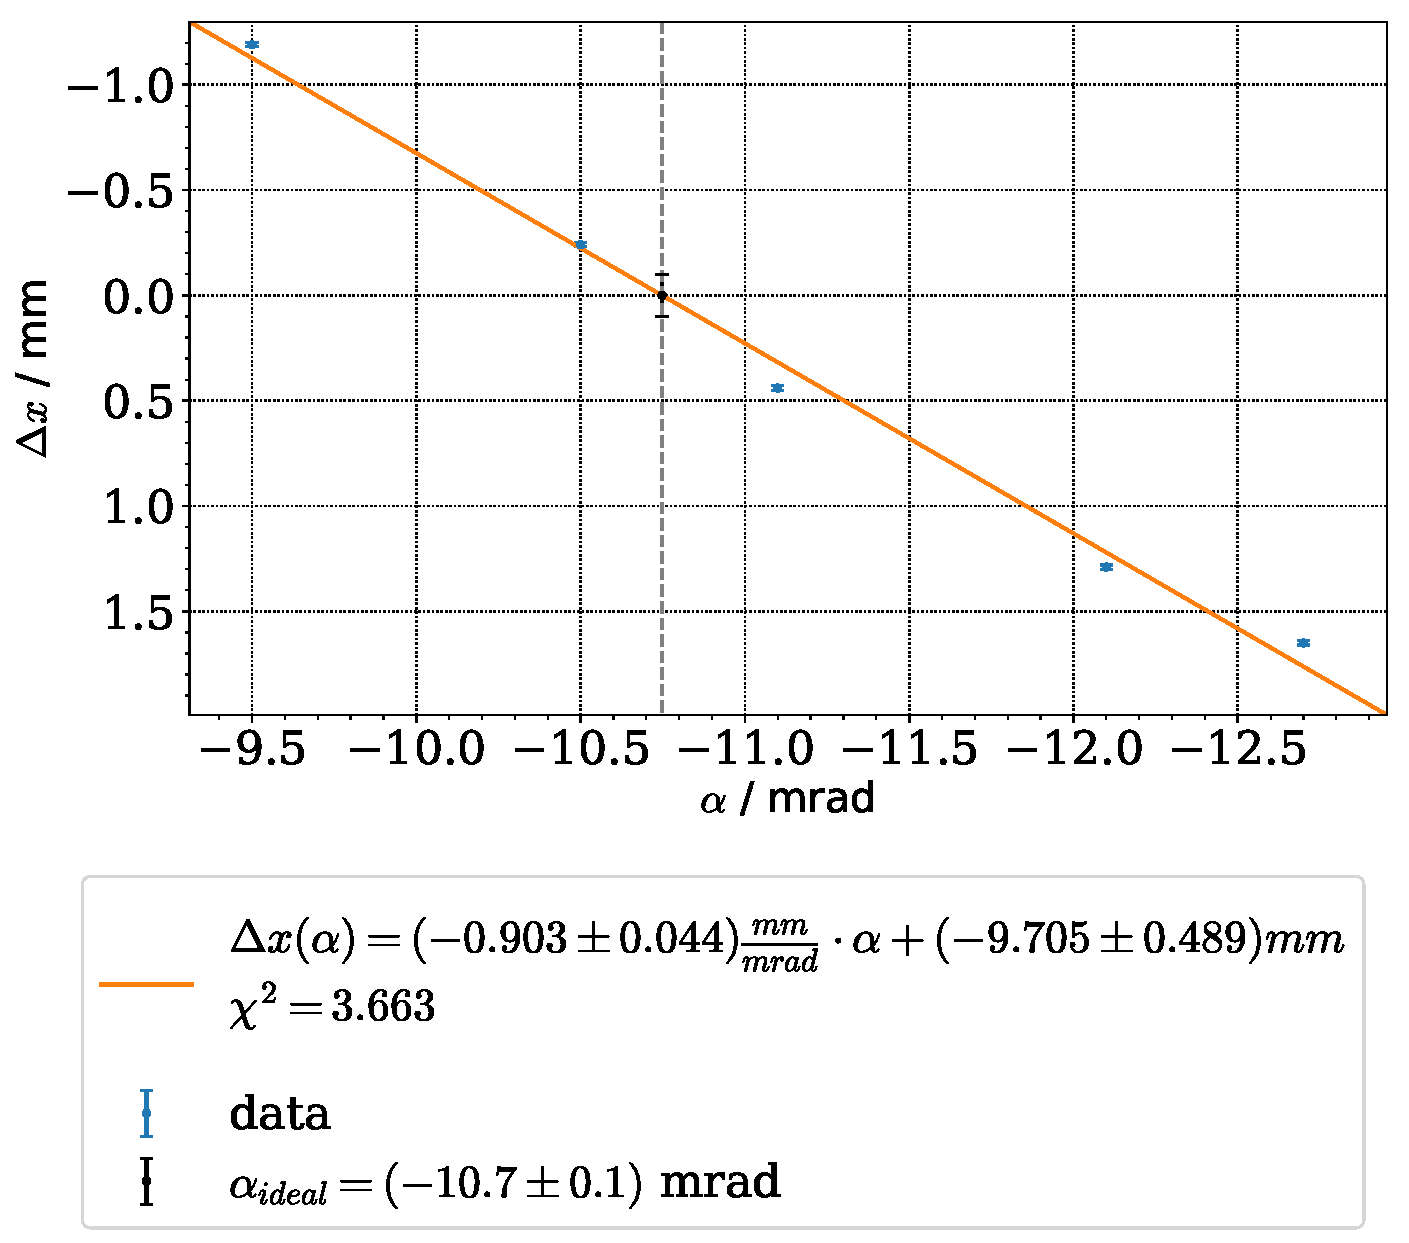
\includegraphics[width=\linewidth]{figs/calibration/q2_x.pdf}
		\caption{$x$-axis, corrector C1}
	\end{subfigure}
	\begin{subfigure}{.49\linewidth}
		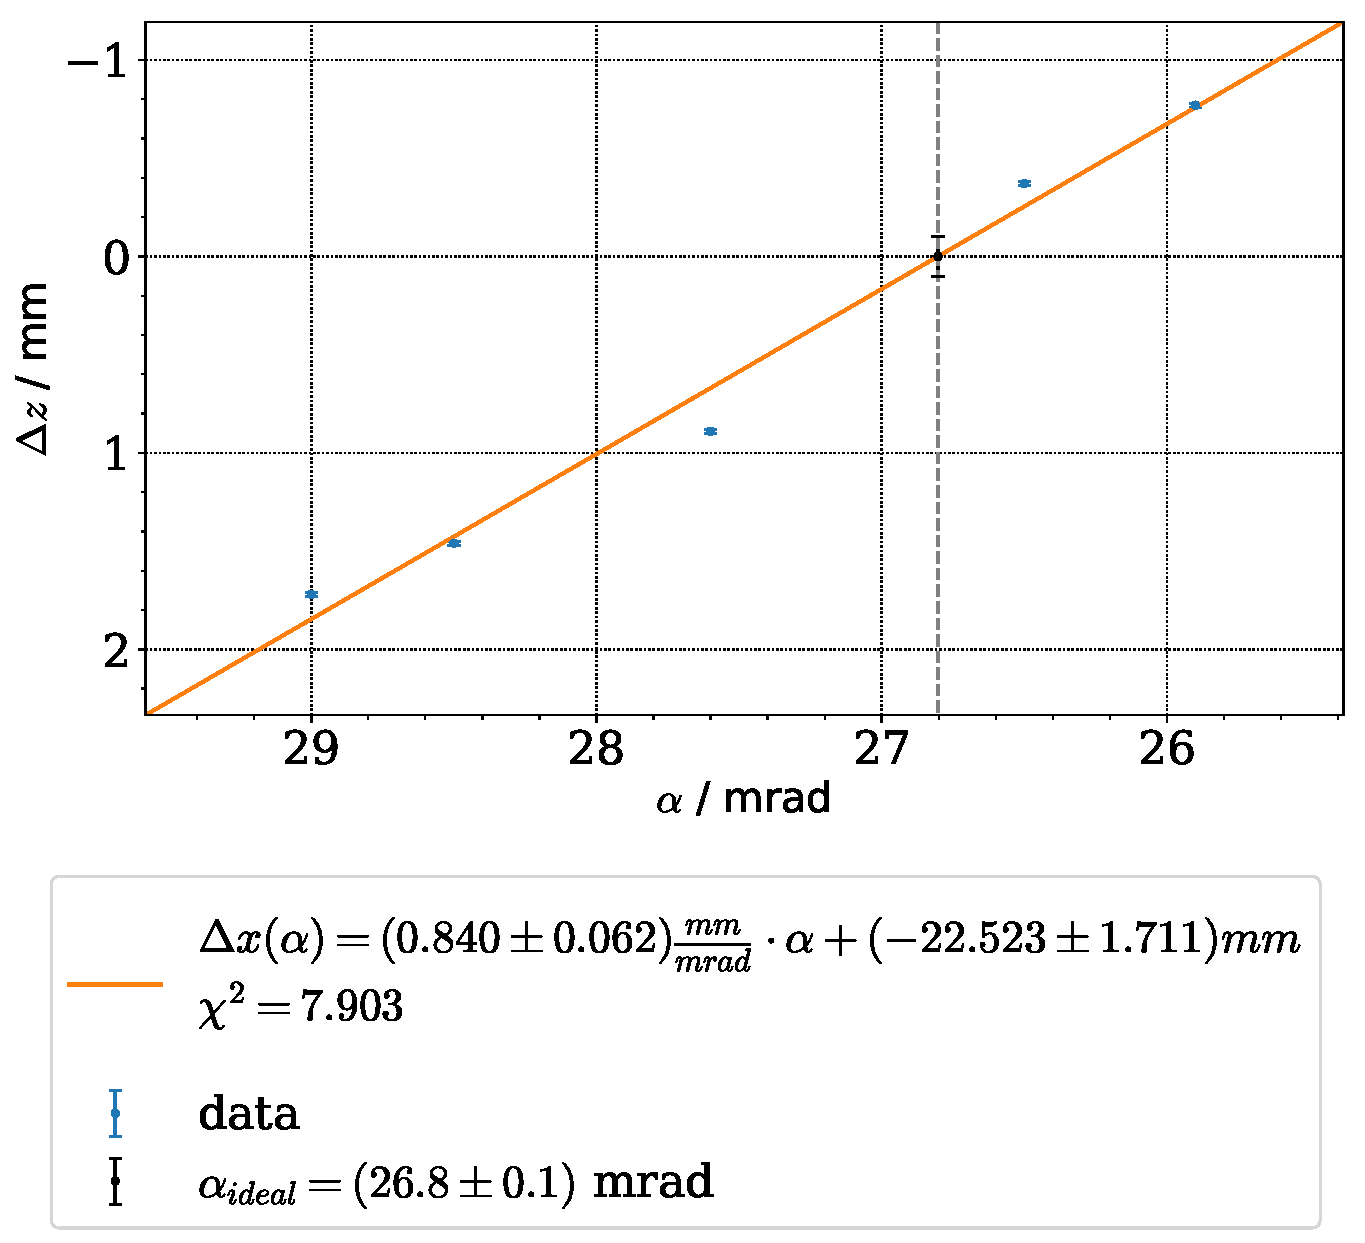
\includegraphics[width=\linewidth]{figs/calibration/q2_z.pdf}
		\caption{$z$-axis, corrector C1}
	\end{subfigure}
		\begin{subfigure}{.49\linewidth}
		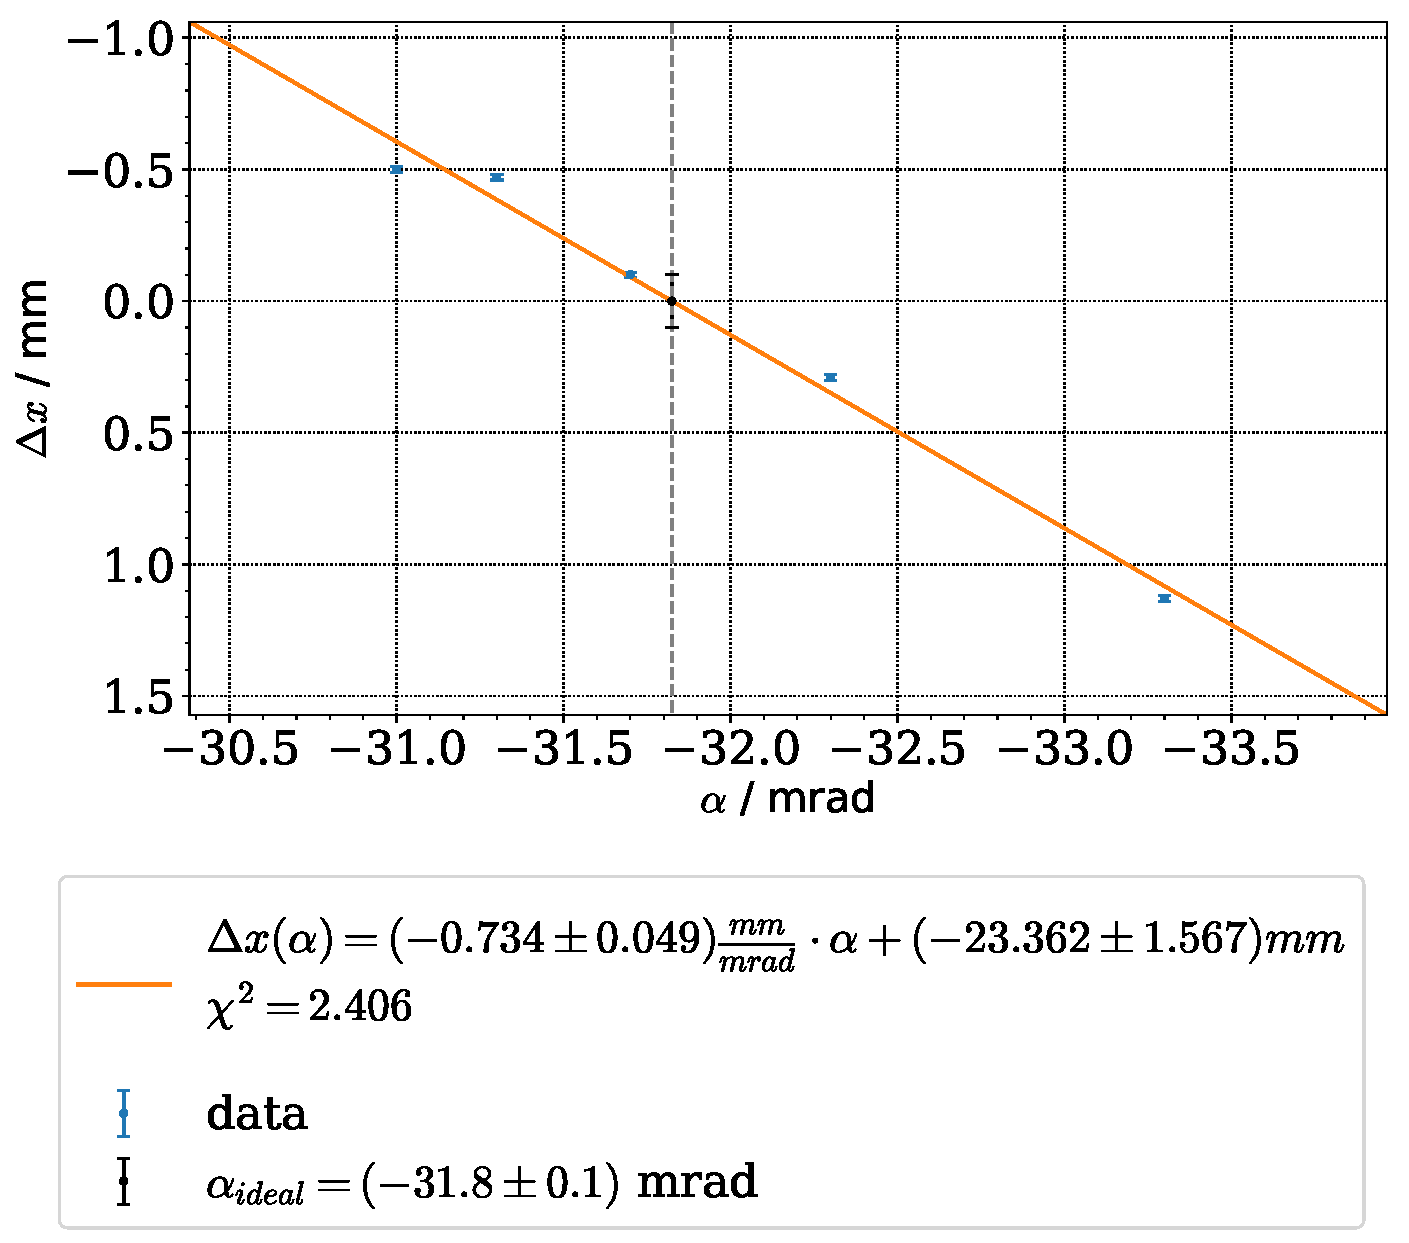
\includegraphics[width=\linewidth]{figs/calibration/q3_x.pdf}
		\caption{$x$-axis, corrector C2}
	\end{subfigure}
	\begin{subfigure}{.49\linewidth}
		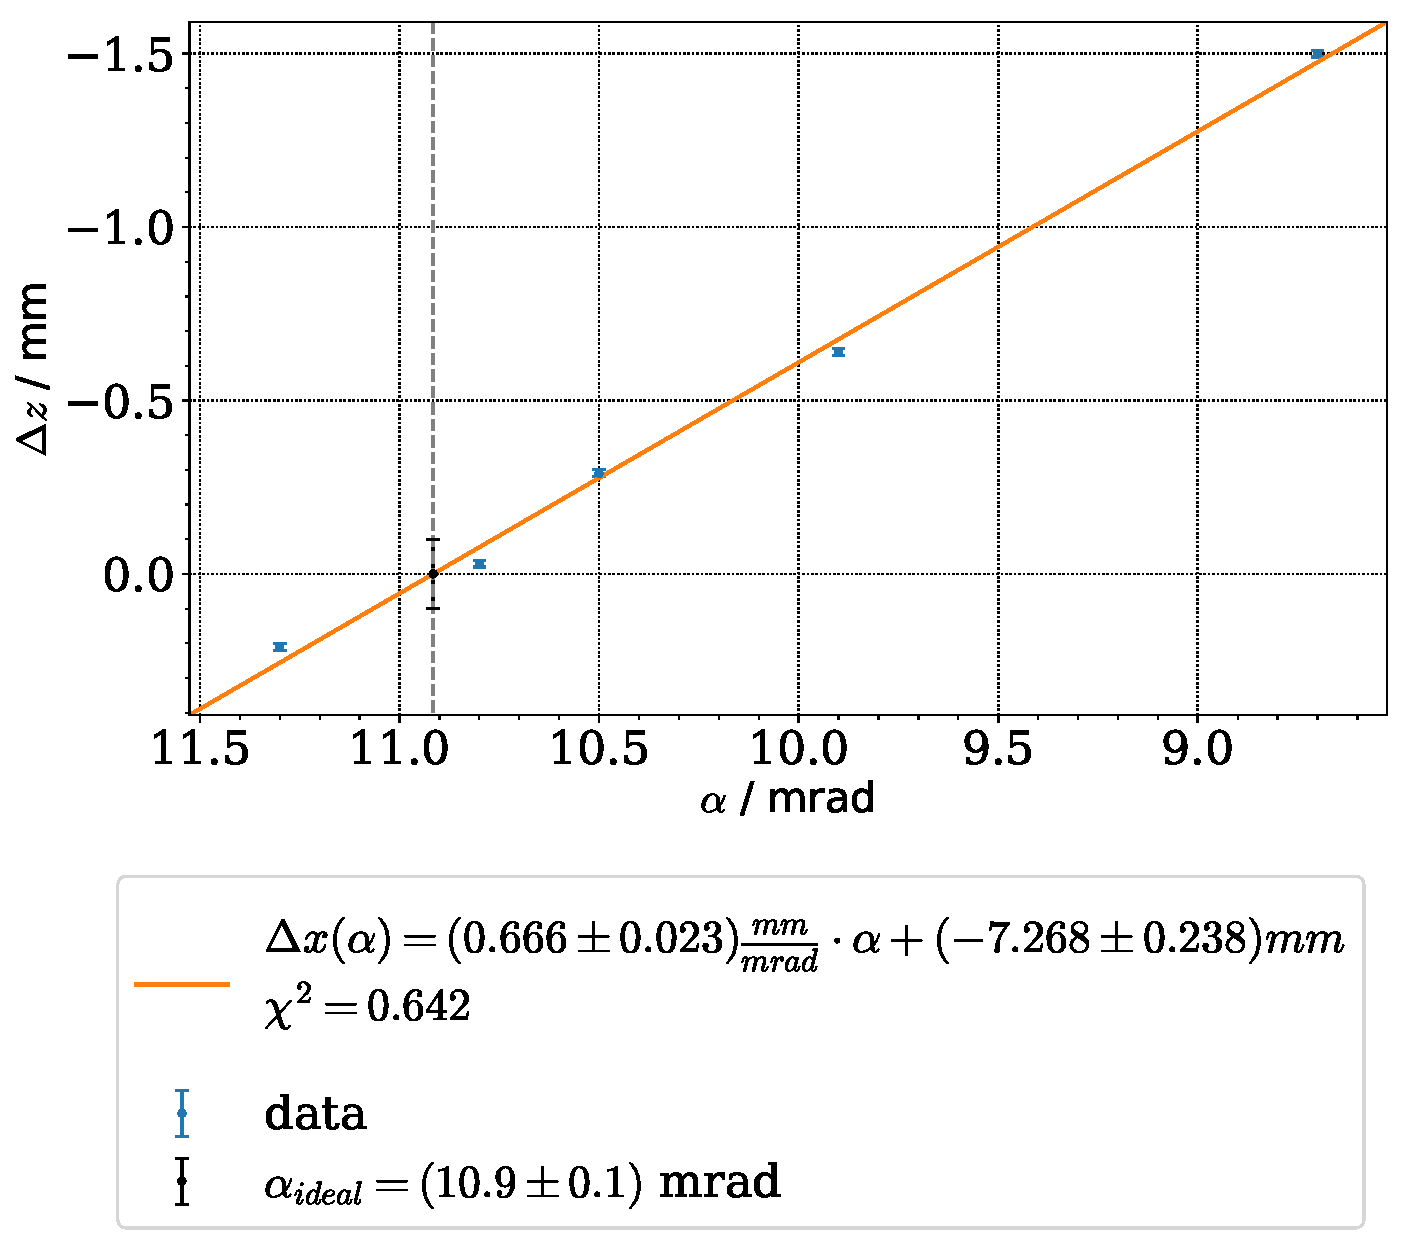
\includegraphics[width=\linewidth]{figs/calibration/q3_z.pdf}
		\caption{$z$-axis, corrector C2}
	\end{subfigure}
	\begin{subfigure}{.49\linewidth}
		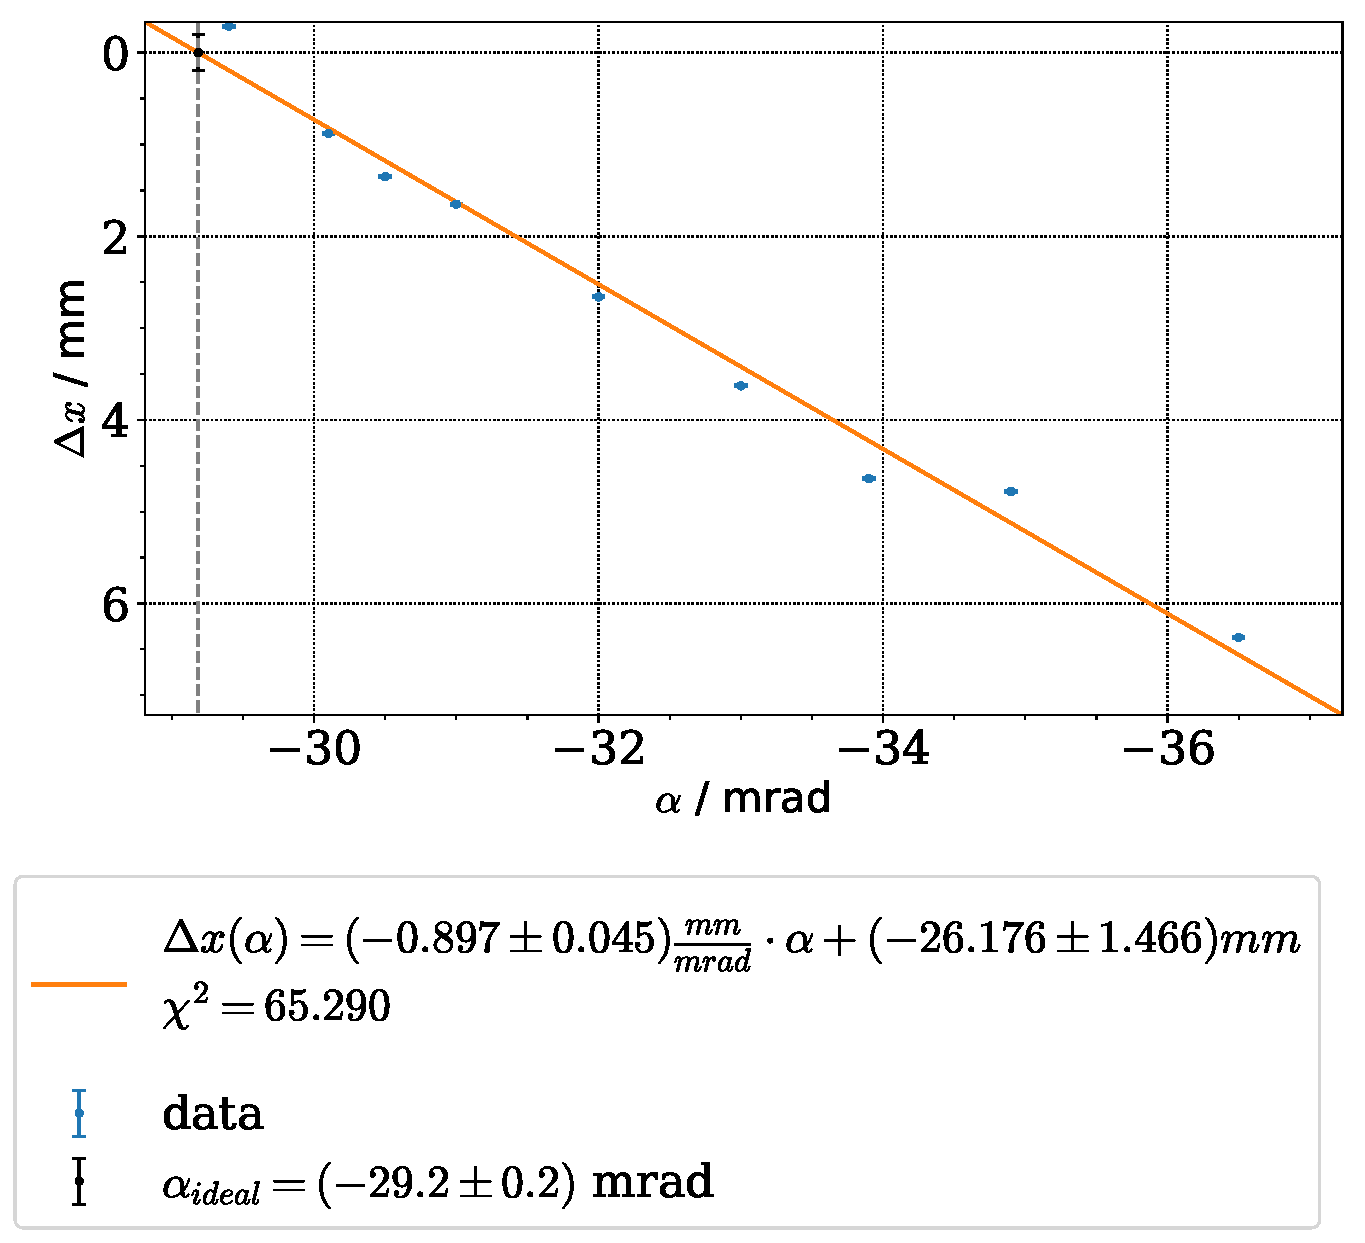
\includegraphics[width=\linewidth]{figs/calibration/q4_x.pdf}
		\caption{$x$-axis, corrector C3}
	\end{subfigure}
	\begin{subfigure}{.49\linewidth}
		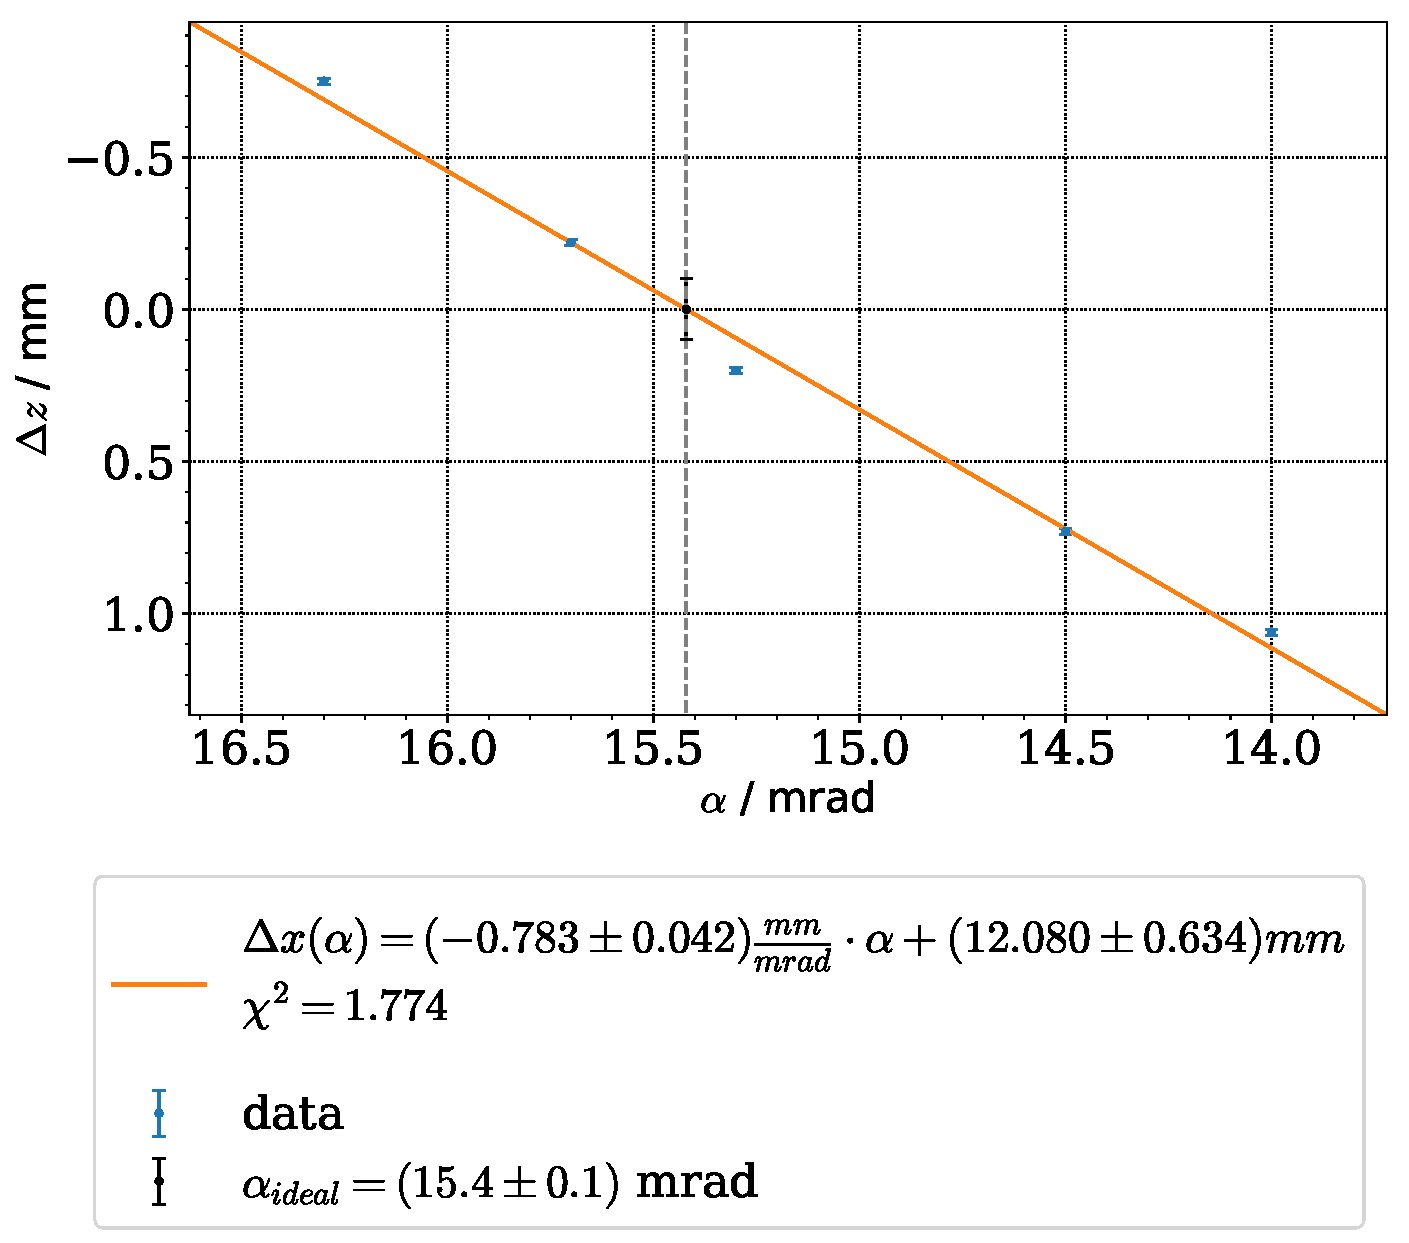
\includegraphics[width=\linewidth]{figs/calibration/q4_z.pdf}
		\caption{$z$-axis, corrector C3}
	\end{subfigure}
	\caption{Beam alignment in the $x$- and $z$-axis for the correctors C1-C3}\label{fig:quad_calib_rest}
\end{figure}
\newpage
\subsection{Measurement data}
Here we list the data we took for the quadrupole scan. In addition to the measured width we provide here statistical and systematical error. The statistical error was estimated based on the fluctuations that the fit procedure yielded. The systematical error is the one discussed in subsection \ref{subsec:err}. The cumulative error is then computed using \textsc{Gaussian} error propagation.
\begin{table}[htbp]
	\centering
	\begin{tabular}{c|c|c|c|c}
		$k / 1/m^2$ & $\sigma_x$ / mm & stat error / mm & sys error / mm & cum error / mm \\
		\hline
		\hline
		0         & 1.35               & 0.03            & 0.14           & 0.143178       \\
		0.8       & 1.35               & 0.03            & 0.14           & 0.143178       \\
		2         & 1.3                & 0.03            & 0.14           & 0.143178       \\
		2.8       & 1.26               & 0.03            & 0.14           & 0.143178       \\
		3.6       & 1.24               & 0.03            & 0.14           & 0.143178       \\
		5.1       & 1.19               & 0.03            & 0.14           & 0.143178       \\
		5.9       & 1.15               & 0.03            & 0.14           & 0.143178       \\
		7.5       & 1.1                & 0.03            & 0.14           & 0.143178       \\
		9.5       & 1.05               & 0.03            & 0.14           & 0.143178       \\
		11.1      & 1                  & 0.03            & 0.14           & 0.143178       \\
		13        & 0.92               & 0.01            & 0.14           & 0.140357       \\
		15.8      & 0.85               & 0.01            & 0.14           & 0.140357       \\
		19        & 0.78               & 0.01            & 0.14           & 0.140357       \\
		24.1      & 0.65               & 0.01            & 0.14           & 0.140357       \\
		28.1      & 0.57               & 0.01            & 0.14           & 0.140357       \\
		32        & 0.52               & 0.01            & 0.14           & 0.140357       \\
		35.2      & 0.5                & 0.01            & 0.14           & 0.140357       \\
		38        & 0.52               & 0.01            & 0.14           & 0.140357       \\
		36        & 0.51               & 0.01            & 0.14           & 0.140357       \\
		34.8      & 0.51               & 0.01            & 0.14           & 0.140357       \\
		33.6      & 0.52               & 0.01            & 0.14           & 0.140357       \\
		38.7      & 0.54               & 0.01            & 0.14           & 0.140357       \\
		39.5      & 0.55               & 0.01            & 0.14           & 0.140357       \\
		41.5      & 0.57               & 0.01            & 0.14           & 0.140357       \\
		43.1      & 0.59               & 0.01            & 0.14           & 0.140357       \\
		46.3      & 0.64               & 0.03            & 0.14           & 0.143178       \\
		48.2      & 0.67               & 0.03            & 0.14           & 0.143178       \\
		52.2      & 0.75               & 0.03            & 0.14           & 0.143178       \\
		58.1      & 0.88               & 0.03            & 0.14           & 0.143178      
	\end{tabular}
\caption{Quadrupole scan at Screen S1 in horizontal direction}
\label{tab:qscan1x}
\end{table}
\begin{table}[htbp]
		\centering
	\begin{tabular}{c|c|c|c|c}
		$k / 1/m^2$ & $\sigma_z$ & stat error / mm & sys error / mm & cum error / mm \\
		\hline
		\hline
		0         & 1.03    & 0.03            & 0.08           & 0.08544        \\
		-3.2      & 0.93    & 0.03            & 0.08           & 0.08544        \\
		-5.1      & 0.88    & 0.03            & 0.08           & 0.08544        \\
		-8.3      & 0.81    & 0.03            & 0.08           & 0.08544        \\
		-10.3     & 0.76    & 0.03            & 0.08           & 0.08544        \\
		-12.3     & 0.71    & 0.03            & 0.08           & 0.08544        \\
		-13.8     & 0.67    & 0.03            & 0.08           & 0.08544        \\
		-16.2     & 0.62    & 0.03            & 0.08           & 0.08544        \\
		-19       & 0.58    & 0.03            & 0.08           & 0.08544        \\
		-20.6     & 0.54    & 0.01            & 0.08           & 0.0806226      \\
		-24.1     & 0.5     & 0.01            & 0.08           & 0.0806226      \\
		-26.5     & 0.49    & 0.01            & 0.08           & 0.0806226      \\
		-30       & 0.5     & 0.01            & 0.08           & 0.0806226      \\
		-28.9     & 0.49    & 0.01            & 0.08           & 0.0806226      \\
		-27.7     & 0.5     & 0.01            & 0.08           & 0.0806226      \\
		-32.4     & 0.52    & 0.01            & 0.08           & 0.0806226      \\
		-34.4     & 0.55    & 0.01            & 0.08           & 0.0806226      \\
		-38       & 0.6     & 0.03            & 0.08           & 0.08544        \\
		-41.1     & 0.66    & 0.03            & 0.08           & 0.08544        \\
		-45.1     & 0.72    & 0.03            & 0.08           & 0.08544        \\
		-48.2     & 0.79    & 0.03            & 0.08           & 0.08544        \\
		-55.4     & 0.95    & 0.03            & 0.08           & 0.08544       
	\end{tabular}
\caption{Quadrupole scan at Screen S1 in vertical direction}
\label{tab:qscan1z}
\end{table}
\begin{table}[htbp]
		\centering
	\begin{tabular}{c|c|c|c|c}
		$k / 1/m^2$ & $\sigma_x$ / mm & stat error / mm & sys error / mm & cum error / mm \\
		\hline
		\hline
		0    & 1.38 & 0.03 & 0.14 & 0.143178 \\
		8.7  & 1.13 & 0.03 & 0.14 & 0.143178 \\
		11.9 & 1.04 & 0.03 & 0.14 & 0.143178 \\
		15   & 0.95 & 0.03 & 0.14 & 0.143178 \\
		18.2 & 0.88 & 0.03 & 0.14 & 0.143178 \\
		20.6 & 0.82 & 0.03 & 0.14 & 0.143178 \\
		25.3 & 0.75 & 0.03 & 0.14 & 0.143178 \\
		29.7 & 0.65 & 0.03 & 0.14 & 0.143178 \\
		34   & 0.61 & 0.03 & 0.14 & 0.143178 \\
		40.3 & 0.58 & 0.01 & 0.14 & 0.140357 \\
		44.3 & 0.57 & 0.01 & 0.14 & 0.140357 \\
		50.2 & 0.6  & 0.01 & 0.14 & 0.140357 \\
		47.4 & 0.6  & 0.01 & 0.14 & 0.140357 \\
		43.9 & 0.57 & 0.01 & 0.14 & 0.140357 \\
		42.7 & 0.56 & 0.01 & 0.14 & 0.140357 \\
		41.9 & 0.56 & 0.01 & 0.14 & 0.140357 \\
		51   & 0.61 & 0.03 & 0.14 & 0.143178 \\
		54.6 & 0.65 & 0.03 & 0.14 & 0.143178 \\
		60.1 & 0.73 & 0.03 & 0.14 & 0.143178 \\
		66.8 & 0.83 & 0.03 & 0.14 & 0.143178 \\
		75.9 & 1    & 0.03 & 0.14 & 0.143178
	\end{tabular}
\caption{Quadrupole scan at Screen S2 in horizontal direction}
\label{tab:qscan2x}
\end{table}
\begin{table}[htbp]
	\centering
	\begin{tabular}{c|c|c|c|c}
		$k / 1/m^2$ & $\sigma_x$ / mm & stat error / mm & sys error / mm & cum error / mm \\
		\hline
		\hline
		0     & 0.95 & 0.03 & 0.07 & 0.0761577 \\
		-6.3  & 0.83 & 0.03 & 0.07 & 0.0761577 \\
		-10.3 & 0.78 & 0.03 & 0.07 & 0.0761577 \\
		-14.2 & 0.71 & 0.03 & 0.07 & 0.0761577 \\
		-19.4 & 0.63 & 0.03 & 0.07 & 0.0761577 \\
		-24.1 & 0.57 & 0.03 & 0.07 & 0.0761577 \\
		-28.5 & 0.53 & 0.03 & 0.07 & 0.0761577 \\
		-33.2 & 0.5  & 0.03 & 0.07 & 0.0761577 \\
		-36.4 & 0.49 & 0.01 & 0.07 & 0.0707107 \\
		-38   & 0.47 & 0.01 & 0.07 & 0.0707107 \\
		-39.9 & 0.47 & 0.01 & 0.07 & 0.0707107 \\
		-42.3 & 0.48 & 0.01 & 0.07 & 0.0707107 \\
		-45.9 & 0.49 & 0.01 & 0.07 & 0.0707107 \\
		-39.1 & 0.48 & 0.01 & 0.07 & 0.0707107 \\
		-37.6 & 0.48 & 0.01 & 0.07 & 0.0707107 \\
		-41.1 & 0.47 & 0.01 & 0.07 & 0.0707107 \\
		-42.7 & 0.48 & 0.01 & 0.07 & 0.0707107 \\
		-44.3 & 0.48 & 0.01 & 0.07 & 0.0707107 \\
		-47.4 & 0.5  & 0.03 & 0.07 & 0.0761577 \\
		-49.8 & 0.51 & 0.03 & 0.07 & 0.0761577 \\
		-52.6 & 0.53 & 0.03 & 0.07 & 0.0761577 \\
		-55   & 0.55 & 0.03 & 0.07 & 0.0761577 \\
		-58.5 & 0.57 & 0.03 & 0.07 & 0.0761577 \\
		-65.2 & 0.62 & 0.03 & 0.07 & 0.0761577 \\
		-70.4 & 0.68 & 0.03 & 0.07 & 0.0761577 \\
		-81.4 & 0.79 & 0.03 & 0.07 & 0.0761577 \\
		-90.5 & 0.9  & 0.03 & 0.07 & 0.0761577
	\end{tabular}
\caption{Quadrupole scan at Screen S2 in vertical direction}
\label{tab:qscan2z}
\end{table}


\newpage
\printbibliography[heading=bibintoc]
\end{document}
